\chapter{Substructure Discovery in Tandem Mass Spectometry Data}
\label{c:background}

\section{Introduction}

In this chapter, we explore the application of probabilistic methods to the discovery of patterns in mass spectrometry fragmentation data. As discussed in Section~\ref{sub:identification-background}, analysis of MS metabolomics data is challenging since many molecules cannot be identified from their mass alone (e.g. isobaric molecules, and isomers) \cite{VanderHooft2013, Kind2006}. Separation by liquid chromatography prior to mass spectrometry can add discriminatory information but does not solve the problem as isomers can exhibit similar chromatographic behavior, and chromatographic retention time is unpredictable. From a tandem-MS set-up, fragmentation spectra can be obtained that are characteristic of the structural composition of the precursor ions that generate them, and through the matching against public spectra library, these fragmentation spectra can be used to annotate the identities of the metabolites present in the sample. However, spectral identification itself cannot completely address the identification problem due to the limited number of reference spectra present in databases (e.g. MassBank, HMDB) that a query spectra can be matched against. 

Following the assumption that each observed spectrum is comprised of one or more such substructures, we propose an unsupervised analysis workflow that reduces the large number of fragmentation spectra to sets of co-occurring molecular fragments and neutral losses. This is accomplished through the application of the Latent Dirichlet Allocation (LDA) model to spectral fragmentation data. The proposed workflow, called 'MS2LDA', converts fragmentation spectra into 'documents' of fragment and neutral loss 'word' features and produces as output the sets of topics shared by documents. In the context of fragmentation data, we define a \textit{Mass2Motif} to be a topic that potentially corresponds to a biochemically-relevant molecular substructure shared by many metabolites. 

The results of MS2LDA analysis allows us to immediately explore the biochemistry present in the sample via the relative abundance of a small number of different molecular substructures that, based on our analysis, are often straightforward to annotate. The presence of shared substructures allows us to group metabolites in a meaningful way even if they do not share a large degree of overall spectral similarity. If many molecules in such a group share a pattern of differential expression, we can hypothesise the cause of the change in abundance without having to identify all of the metabolites and map them to a metabolic pathway. Presence of substructures can also be used to provide putative annotations (or functional classifications) for metabolites that are otherwise unidentifiable. We also demonstrate with examples how changes to the expression levels of substructures can be examined from the resulting output of MS2LDA. 

Finally, from the results of performing independent multiple MS2LDA structural annotations on different biological samples, we propose an extension to the standard LDA model that allows the sharing of topics across multiple runs. The extended model allows the presence of topics to be jointly inferred across multiple runs at once, thus eliminating the needs for the tedious matching of topics that occur across runs manually.

\section{Related Work}

Recurring patterns of fragments (product ions) and neutral losses that are present in fragmentation spectra can be explained by the presence of common biological substructures (e.g. a hexose unit, or a CO loss) in metabolites. The representation of small molecules as combinations of building blocks has previously been used for the annotation of a small number of molecules in direct infusion-MS with fragmentation \cite{Sweeney2014} and for metabolite classification in GC-MS \cite{Scott1994, Hummel2010}. CSI:FingerID ranks candidate molecules based on the presence and absence of various predefined structural features, including substructures \cite{Duhrkop2015}. These studies reveal the potential of substructure-based approaches in MS but require structurally known training data, which is costly to produce and often platform-specific. 

Tools exist that operate on the entire fragmentation spectra. For example, “Molecular Networking” clusters MS1 peaks by their MS2 spectral similarity such that one identifiable metabolite in a cluster facilitates structural annotation of its neighbors \cite{yang2013molecular, van2016urinary}.  However, spectral features causing the clustering must be extracted manually and only MS2 spectra with high overall spectral similarity are grouped. Another package, MS2Analyzer \cite{ma2014ms2analyzer} mines MS2 spectra for specific features defined by the user (i.e., mass fragments and neutral losses). Some will be common to many experiments (e.g. CO or H2O losses), but sample-specific features are easily overlooked. Whilst Molecular Networking requires no user intervention it may fail to group molecules that share small substructures, whilst MS2Analyzer can find all molecules that share a particular set of features provided they are user-specified. 

Our approach, MS2LDA, which is based on Latent Dirichlet Allocation (described in Section~\ref{background-lda}) retains the benefits of entire spectra-oriented tools whilst losing the shortfalls – it can find relevant substructures based on the co-occurrence of mass fragments and neutral losses, and group the molecules accordingly. LDA was previously adapted to other types of high throughput data (genomics \cite{chen2010probabilistic}, metagenomics \cite{zhang2015exploiting}, and transcriptomics \cite{rogers2005latent}) but never before to exploit the parallels between MS2 fragmentation data and text.

\section{A Workflow for Substructure Discoveries and Annotations}

As introduced earlier, the key insight to the MS2LDA workflow lies in the parallels between text and MS fragmentation data (Figure~\ref{fig:text2frags}). As a text analysis pipeline relying on LDA decomposes documents into topics based on frequently co-occurring words, so MS2LDA decomposes fragmentation spectra into their constituent building blocks of frequently co-occurring fragments and neutral losses (referred to as ‘Mass2Motifs’). Crucially, MS2LDA achieves this with an unsupervised manner, using all of the fragmentation spectra generated by data-dependent mass fragmentation analysis (DDA) to learn potentially conserved substructures and the decomposition of the fragmentation spectra into those substructures. 

\begin{figure}[!htbp]
\centering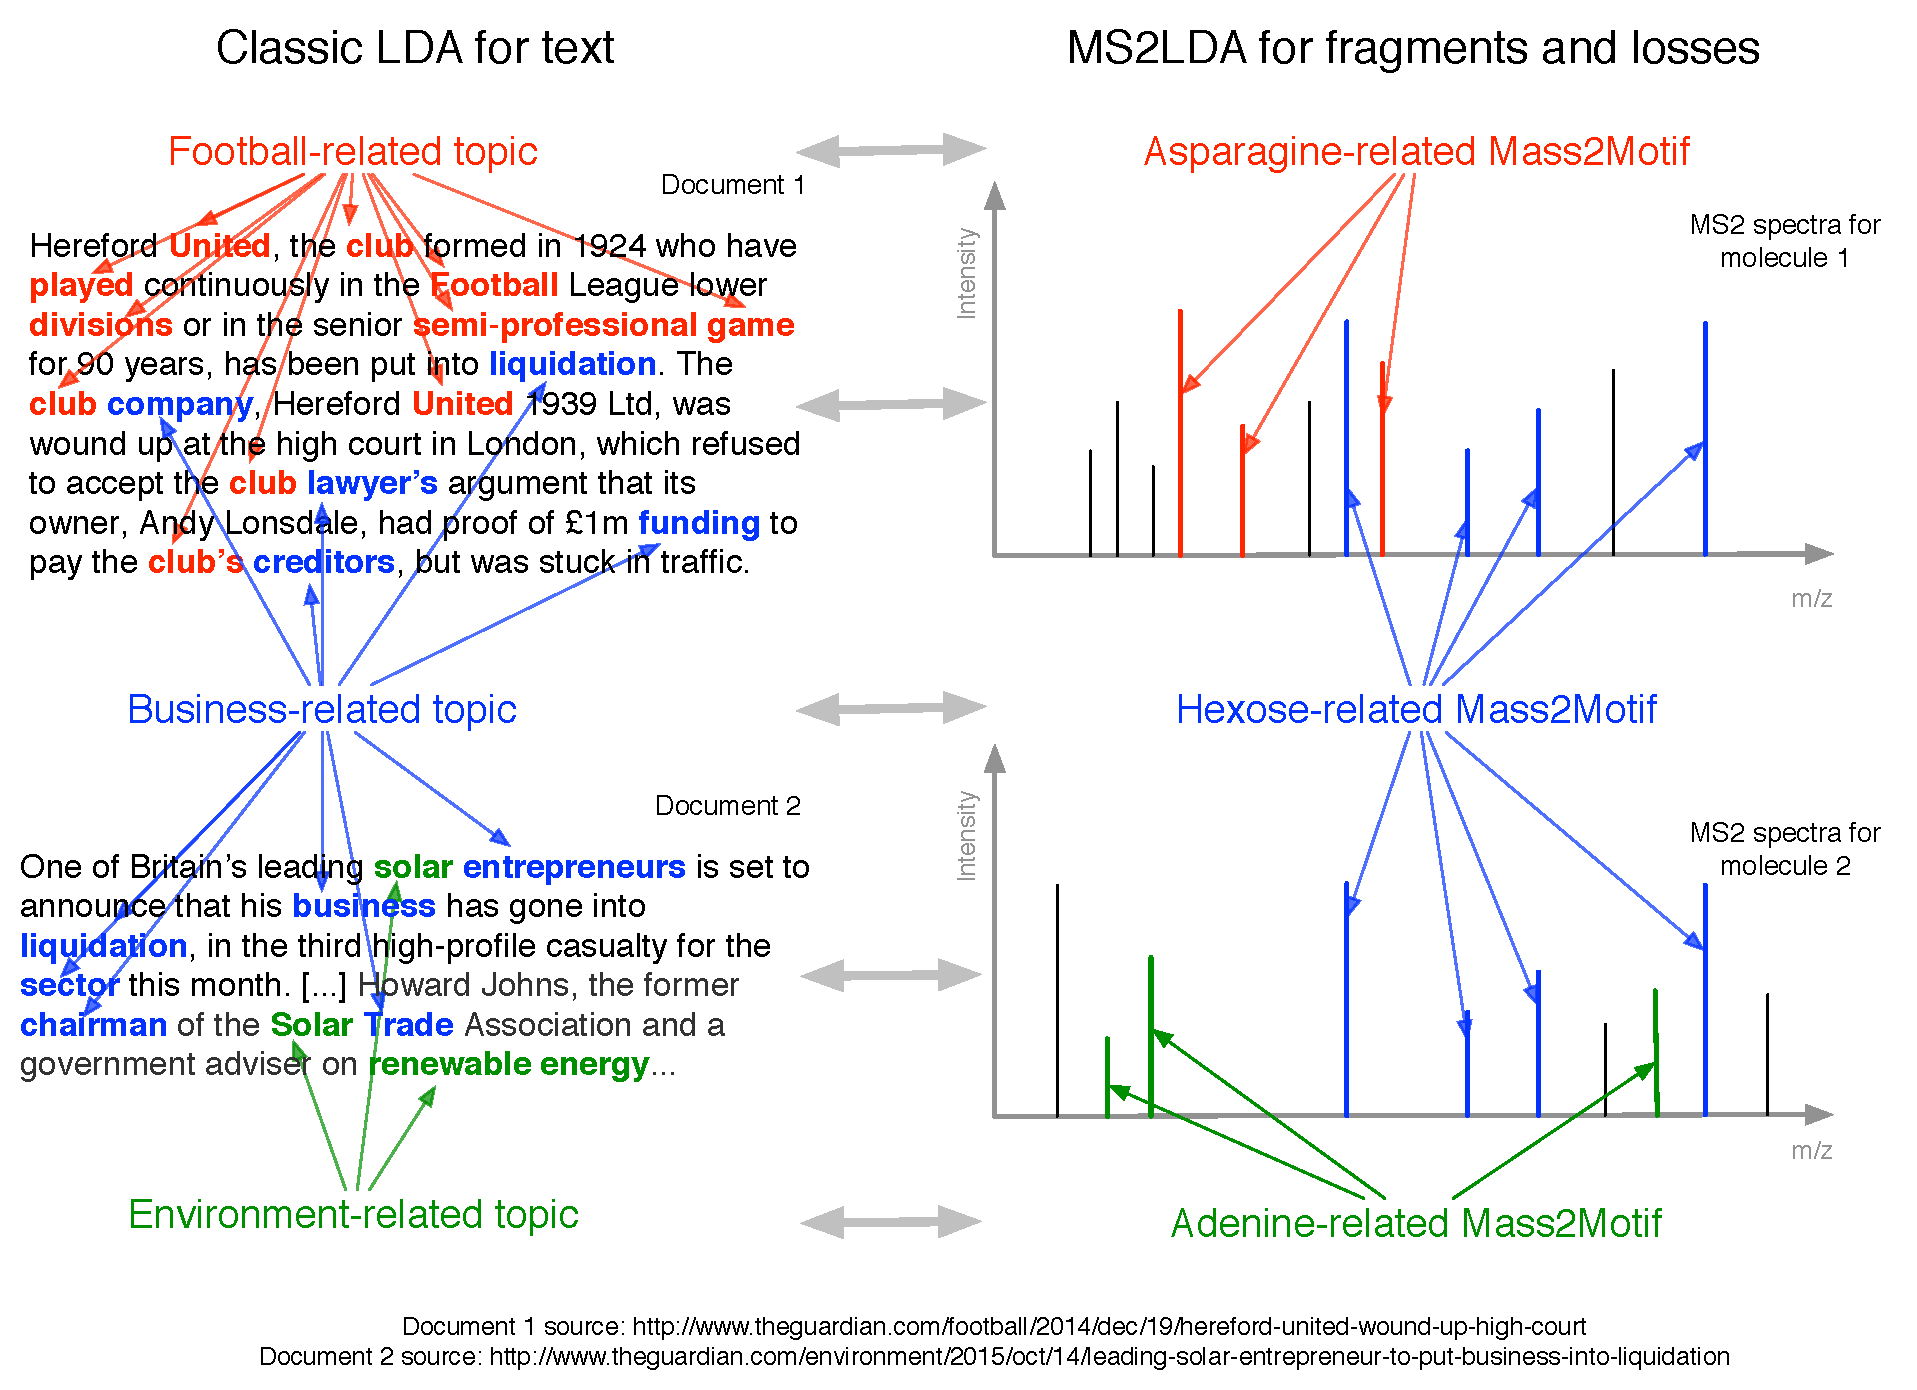
\includegraphics[width=0.7\linewidth]{07-lda/figures/text2frags.pdf}
\centering\caption{Figure 1: Analogy between LDA for text-mining and MS2LDA. In this example, we can see that traditional LDA has extracted topics that can be interpreted as ‘football related’, ‘business-related’ and ‘environment related’. Each document is a combination of different topics. In a similar manner, MS2LDA extracts different sets of concurring mass fragments or losses (Mass2Motifs) from the fragmentation spectra of precursor ions that can be interpreted as ‘Asparagine-related’, ‘Hexose-related’ and ‘Adenine-related’. Each fragmentation spectra is made up of one or more Mass2Motifs.\label{fig:text2frags}}
\end{figure}

The MS2LDA workflow consists of two stages: i) the data conversion stage, which prepares the acquired fragmentation data into suitable input format for the workflow, followed by ii) the Mass2Motif discovery stage, which performs topic modelling via LDA to discover mass fragmental patterns, assigns potential candidate elemental formulae to MS1 and MS2 peaks, and visualises the Mass2Motifs in an interactive environment. The complete workflow is schematically illustrated in Figure~\ref{fig:m2lda-workflow} and described in more details in the following Section~\ref{sub:data-conversion} and \ref{sub:topic-discovery}.

\begin{figure}[!htbp]
\centering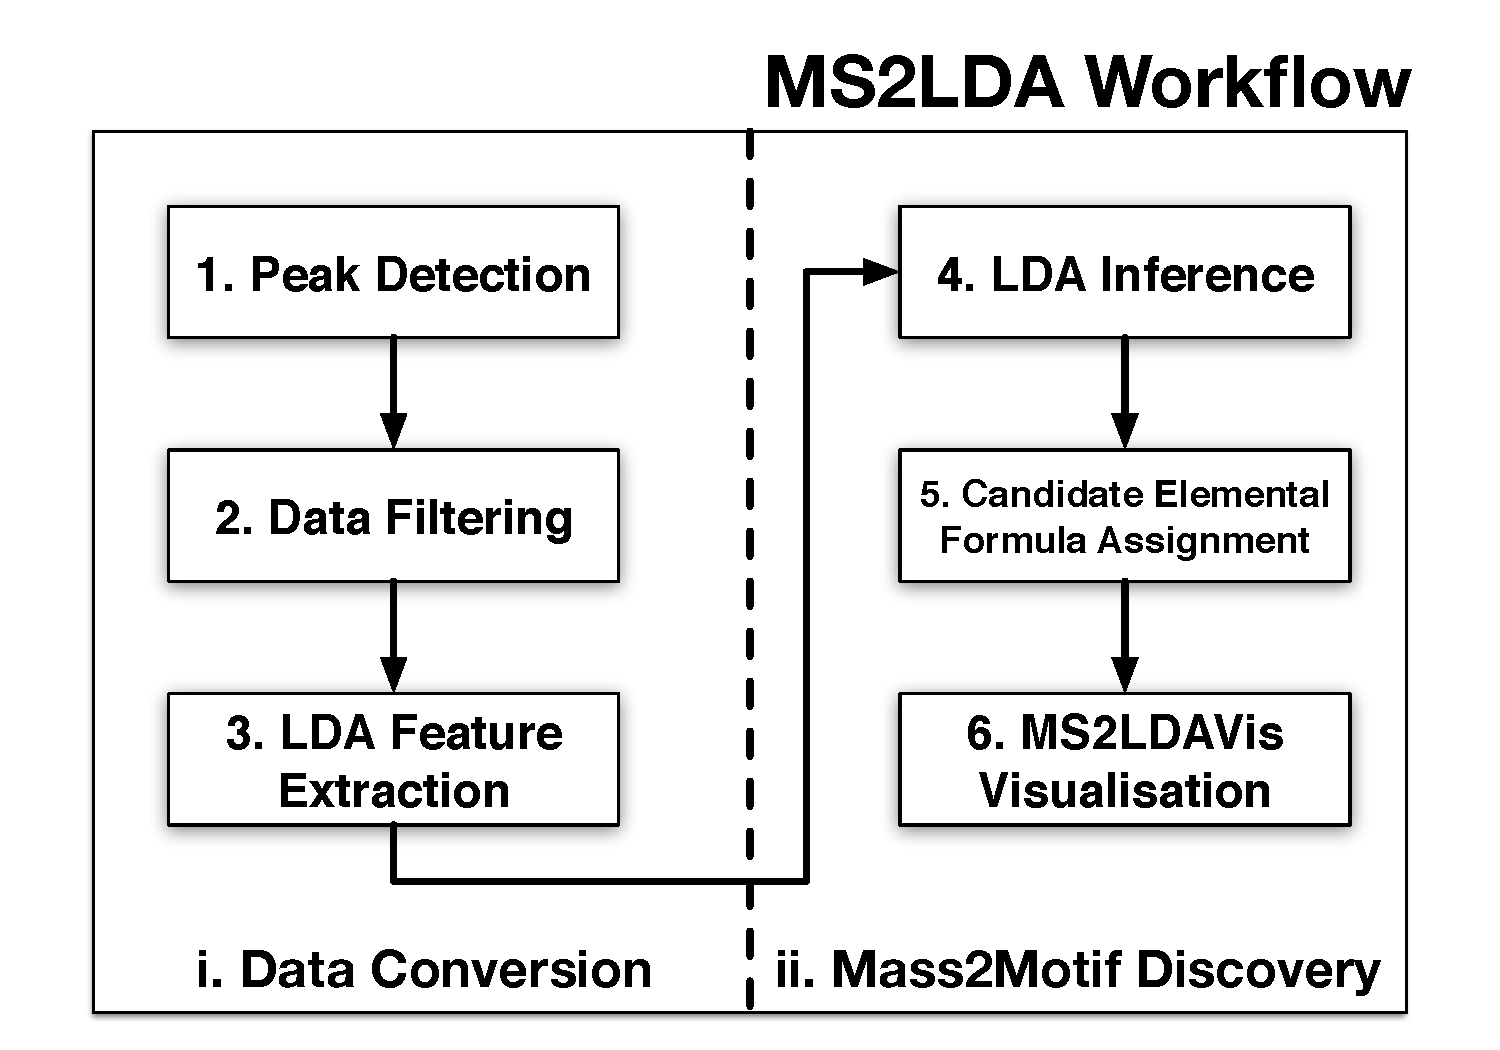
\includegraphics[width=0.8\linewidth]{07-lda/figures/ms2lda.pdf}
\centering\caption{Schematic overview of the MS2LDA workflow..\label{fig:m2lda-workflow}}
\end{figure}

\subsection{Data Conversion\label{sub:data-conversion}}

\subsubsection{Peak Detection \& Data Filtering}

Data conversion is an essential part of the MS2LDA workflow, since the acquired fragmentation data cannot readily be used for the purpose of mass fragmental pattern searching. As input, Our workflow accepts the combination of a single full-scan file for the MS1 peaks and a separate fragmentation file for the MS2 peaks. The data conversion process starts with the detection of MS1 peak in the input .mzXML file obtained from full-scan mode spectra using the CentWave algorithm from the XCMS library \cite{Smith2006}. This constitutes information on the MS1-level. Fragmentation data, in the form of .mzML file obtained from tandem MS mode, are processed using an R script based on the RMassBank package \cite{Stravs2013}. The script performs a greedy search for the most intense unique MS2 spectrum that can be linked to an MS1 LC-MS peak within a specified retention time (RT) window. A filtering step based on RT and intensity is applied to remove noisy peaks, as well as the washing part, equilibration part, and the start of the chromatogram prior to the injection peak. Any MS1 peak not having paired MS2 peaks is subsequently discarded for further processing. The aim of the filtering step is to exclude identical fragmentation spectra produced by low-intensity MS1 peaks that were fragmented multiple times, which could potentially forming a topic on their own. 

\subsubsection{LDA Feature Extraction}

The next step in the data conversion stage is the transformation of the spectral data into a suitable input format, which is a matrix consisting of the MS1 peaks (columns) and their correspondent MS2 word features (rows) (see Figure~\ref{fig:m2lda-matrix}). In LDA applied to the text domain, this corresponds to the matrix of counts of word occurrences in documents. Similarly, each MS1 peak can now be seen as a ‘document’ while the linked MS2 spectrum associated to each MS1 peak produce the ‘word’ features in a document. Following the bag-of-words assumption, LDA does not take into account the word order, but merely the number of times a word occurs in a document. 

\begin{figure}[!htbp]
\centering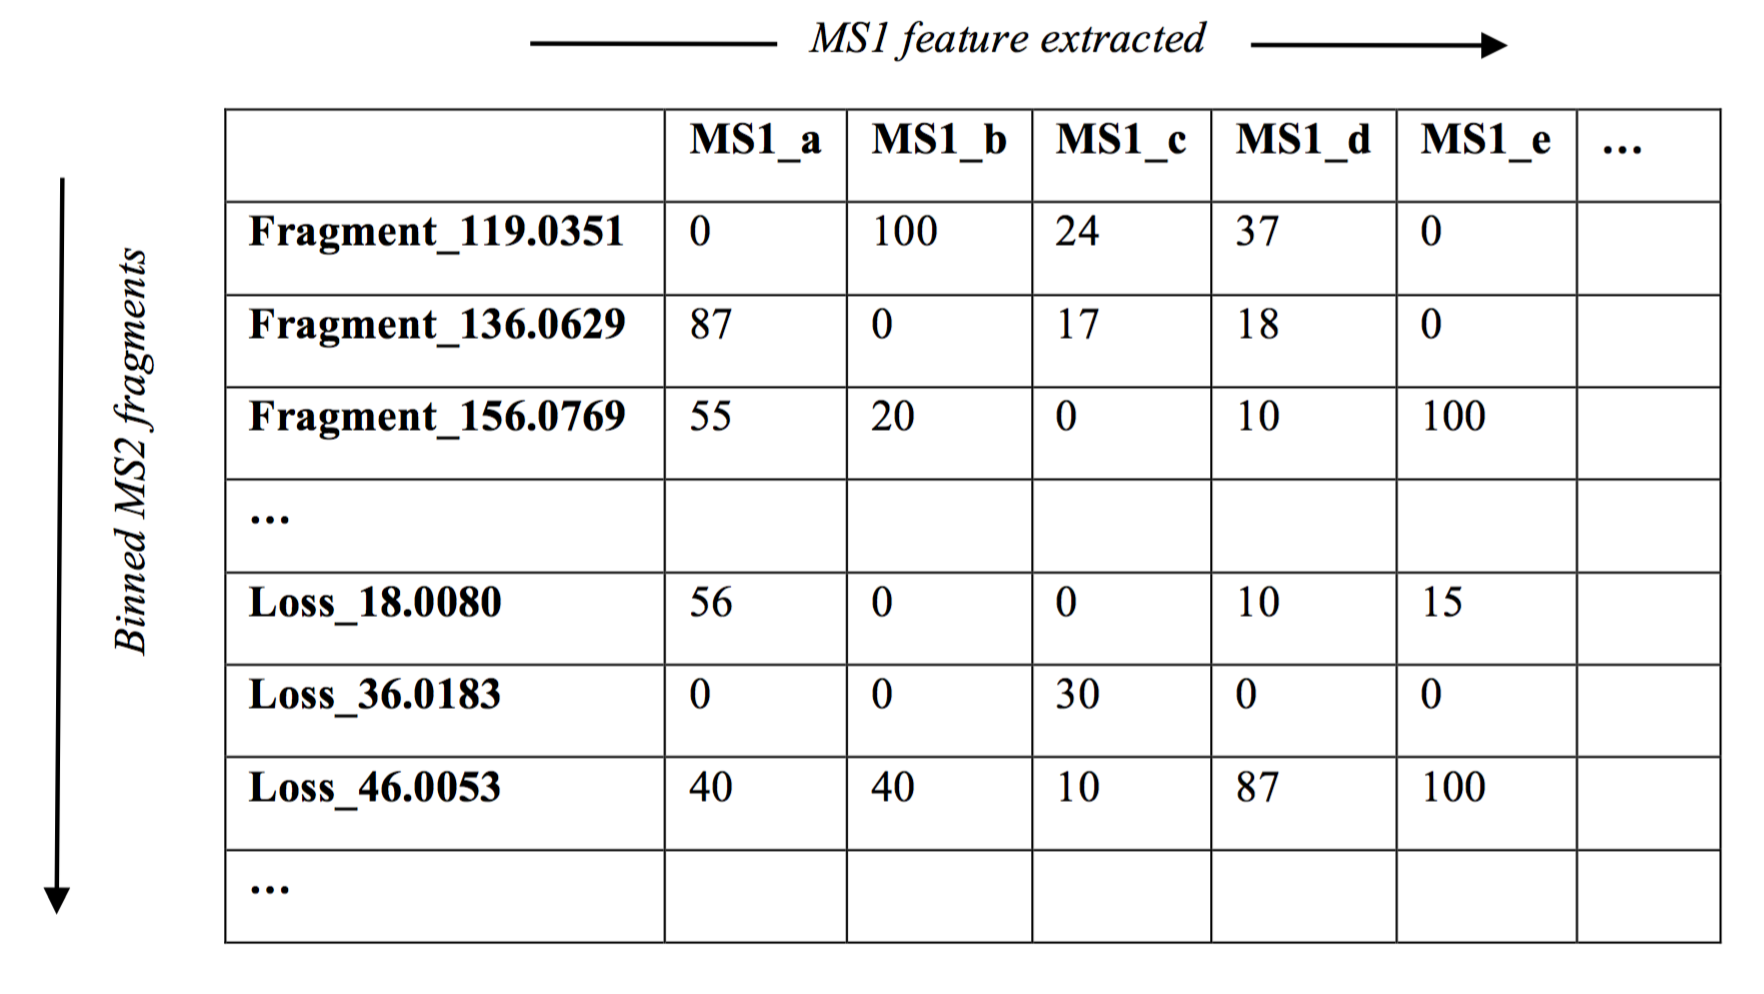
\includegraphics[width=0.8\linewidth]{07-lda/figures/matrix.png}
\centering\caption{The data-frame extracted from fragmentation data: a matrix of XCMS-picked MS1 peaks (columns) and binned mass fragment (and neutral loss) features with normalized (0 – 100 scale) intensities.\label{fig:m2lda-matrix}}
\end{figure}

For each MS1 peak, two types of word features can be extracted from the MS2 fragmentation spectrum:
\begin{itemize}
\item \textbf{Fragment features}, which are the discretized mass values of the MS2 peaks. A greedy binning process is used to group MS2 peaks within a certain user-defined m/z window from the next unprocessed MS2 peak. This way, MS2 peaks with close-enough m/z values but observed in different precursor MS1 peaks are linked and placed into the same discrete bin – each bin corresponds to a fragment feature. The input for inference in textual LDA is the count of occurrences of words in each document; in MS2LDA, the intensity values of MS2 peaks can be considered to be proxies for word counts. These intensity values are normalized by dividing to the largest intensity value in the fragmentation spectrum and discretized on a scale of 0 to 100 (integers). 
\item \textbf{Loss features}, which is the discretized mass values of the neutral losses. Neutral losses are the mass differences between a precursor MS1 peak and each of its MS2 peaks in the spectrum. To produce the loss features, we find the m/z difference between each fragment peak to its precursor ion. Similar to fragment features, the normalized intensity values of the neutral losses, represented by the intensities of their resulting mass fragments, are used as proxies for the loss counts.
\end{itemize}

\subsection{Mass2Motif Discovery\label{sub:topic-discovery}}

\subsubsection{LDA Inference}

After the data conversion step, the resulting matrix has MS2 features (fragments and losses) as rows and columns corresponding to the MS1 peaks. The values in the matrix are the MS2 feature intensities which are subsequently turned into integer counts by normalising and rounding such that the most intense feature for each MS1 peak has value 100. LDA is implemented in Python and uses collapsed Gibbs sampling for inference, the output of which is a set of Mass2Motifs and assignments of Mass2Motifs to each MS1 peak. 

....

\subsubsection{Candidate Elemental Formula Assignment}

To aid with data interpretaton, putative elemental formulae can be displayed alongside the plots of fragmentation spectra explained by a certain Mass2Motif (top-right panel, Figure~\ref{ms2lda-main}). The MS2LDA workflow provides two optional methods to assign candidate elemental formulae to the mass fragments, neutral losses, and precursor ions.  The first is achieved by integrating SIRIUS \cite{Bocker2009} into our workflow. SIRIUS assigns elemental formula by posing it as an integer decomposition problem and solving it through a dynamic programming approach ('Round Robin') \cite{Bocker2007}. SIRIUS is freely-available and, as it is written in Java, can in theory be run platform-independently on any Windows, Unix and Mac environment (in practice, library dependencies have to be satisfied before SIRIUS can be run on the target computer). Integration of SIRIUS into our workflow is achieved by wrapping calls to the Java package of SIRIUS through a separate sub-process, passing it a temporary MGF file that corresponds to each fragmentation spectrum. SIRIUS assigns elemental formulae to each combination of MS1 and MS2 peaks independently, which may lead to mass fragments of similar m/z value being assigned an elemental formula in some spectra, but not in all.

As an alternative strategy for annotation, our workflow also provides a pure Python implementation of an elemental formula assigner (called 'EF-Assigner') based on the Round Robin algorithm that also lies at the heart of SIRIUS. Once the initial assignment of potential candidate formulae to mass fragments, neutral losses and also precursor ion masses has been performed, the list of candidate formulae is further filtered using our implementation of the 7-golden rules, a set of heuristic rules introduced in \cite{Kind2007}. This filtering step is used to remove chemically-unlikely elemental formula compositions from the candidate list. Advantages of the EF-Assigner module are its easy compatibility (it is also written in Python) and it assigns elemental formulae to the binned fragments and losses in the matrix instead of to individual spectra. However, unlike SIRIUS that uses the complete information of the precursor ion and fragments peaks in a spectrum for annotation, EF-Assigner assigns the elemental formulae for the MS1 peaks, mass fragments and neutral losses independently. 

\subsubsection{MS2LDAVis Visualisation}

Due to its hypothesis-generating nature, the analysis of Mass2Motifs to examine if they correspond to actual biochemical substructures is an iterative and exploratory process. In our workflow, this is made possible through the MS2LDAVis module -- an interactive web-based visualization build upon the combination of the Javascript/D3 library and Python to explore and validate Mass2Motifs in fragmentation data. MS2LDAVis is extended from the Python port of the topic modelling visualization interface LDAVis \cite{Sievert2014} used in the text domain, but our adaption in form of MS2LDAVis introduces visualisation features to aid in the exploration of fragmentation data..

Similar to the original LDAVis, the left panel of our MS2LDAVis module shows a global view of the model, whilst the right panel zooms into a specific Mass2Motif (see Figure~\ref{fig:m2ldavis-main}). However, unlike LDAVis where topics are displayed on the left panel through multidimensional scaling that projects topics to two dimensions, the two axes in our MS2LDAVis panel are the log-degree and the $h$-index of Mass2Motifs. We defined the \textit{degree} of a Mass2Motif as the number of fragmentation spectra explained by the Mass2Motif at the user-defined thresholding level $t_{\theta}$ on the fragmentation-spectra-to-Mass2Motif distributions (the $\theta$ parameters). The $h$-index of a Mass2Motif is defined in a similar manner to the conventional $h$-index for scientific publications of a researcher. A Mass2Motif has an index of $h$ if it has $h$ fragment or loss features obtained after setting a user-defined threshold $t_{\phi}$ on the Mass2Motif-to-word distributions (the $\phi$ parameters), each of which occur in the set of thresholded documents at least $h$ times. Intuitively, Mass2Motif with high degrees but low $h$-index could potentially correspond to simple structural features or substructures that occur in many MS2 fragmentation spectra, while Mass2Motif with high $h$-index but lower degrees could potentially correspond to more unique and complex substructures shared by fewer MS2 spectra.

\begin{figure}[!htbp]
\centering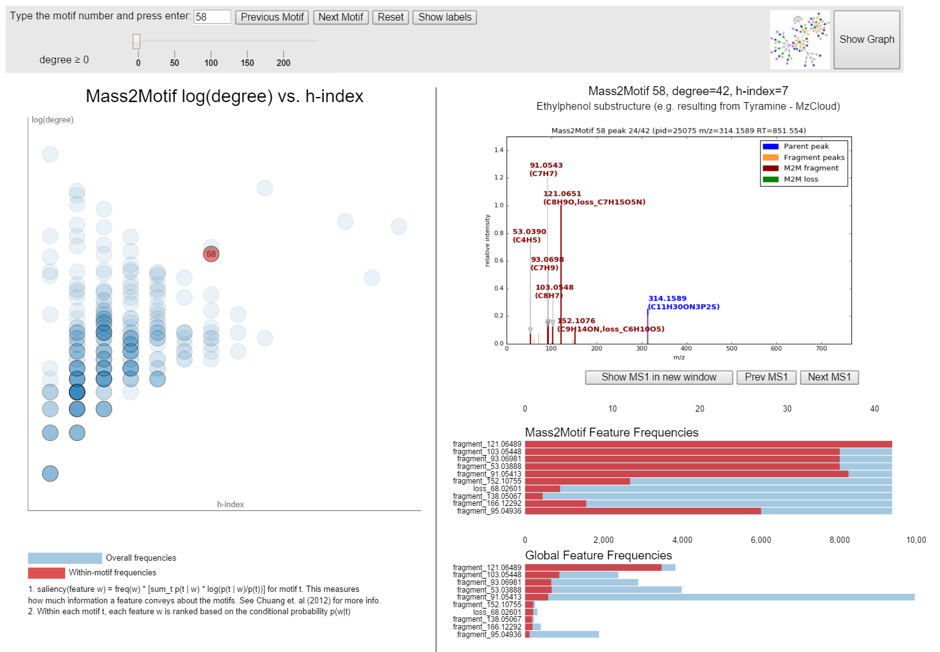
\includegraphics[width=1.0\linewidth]{07-lda/figures/ms2ldavis.png}
\centering\caption{Screenshot of MS2LDAVis. See text for explanations of the different panels.\label{fig:m2ldavis-main}}
\end{figure}

Similar to LDAVis, the left and right panels of our visualization are linked such that selecting a Mass2Motif on the left changes the information displayed on the right panel. We further enhanced MS2LDAVis by plotting the fragmentation spectra of each MS1 peak (documents) above the user-defined threshold  in the selected Mass2Motif. The fragment and loss words in the fragmentation spectra that are explained by the currently selected Mass2Motif, i.e., above the user-defined threshold , are highlighted in bold and user can easily flip through different fragmentation spectra explained by the topic by clicking the ‘Previous MS1’ and ‘Next MS1’ buttons. The bottom of the right panel displays two feature frequency histograms; the Mass2Motif Feature Frequencies histogram displays the counts of each Mass2Motif associated fragment or loss (above the user-defined threshold  on the Mass2Motif-to-word distributions [the φ parameters]) within the fragmentation spectra explained by the Mass2Motif. Similarly, the Global Feature Frequencies histogram display the overall frequency of the fragments or losses within the complete data set that can be explained by the currently selected Mass2Motif. This provides an estimate of how unique the fragment/loss features are in the whole data set.

Finally, to complement our main view, we also allow the possibility of exploring the inferred substructure data in a pop-up network graph (Figure~\ref{fig:m2ldavis-popup}), where Mass2Motifs and MS1 peaks form the nodes in the graph and edges are drawn between them if a document is explained by a topic with conditional probability above the user-defined threshold . The graph view can be accessed by clicking on the ‘Show Graph’ button in the main visualization window. To minimize clutter in the network graph, user can also define a threshold on the degree of the Mass2Motifs, i.e., all Mass2Motifs with a degree of 10 or lower can easily be removed from the graph. Nodes in the graph can also be annotated and coloured according to user-defined specifications before the visualisation interface is called. The two complementary views are linked such that clicking a topic node on the network graph will select the corresponding topic on the main view and vice versa. The network graph is particularly useful in exploring the relationships between Mass2Motifs and investigating which MS1 peaks have fragmentation spectra that can be explained by multiple Mass2Motifs.

\begin{figure}[!htbp]
\centering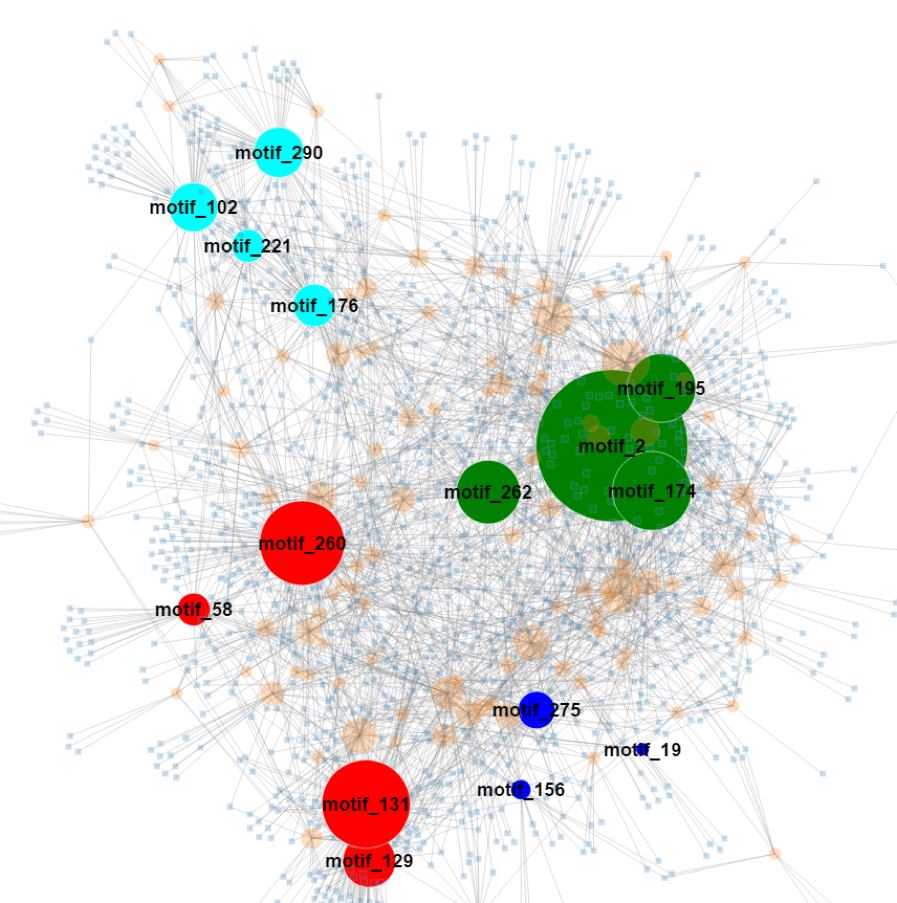
\includegraphics[width=0.8\linewidth]{07-lda/figures/popup.png}
\centering\caption{MS2LDAVis network graph of beer3 extract positive ionization mode file where a number of Mass2Motifs were selectively colored before loading the network visualization. Mass2Motifs circles are proportional to their degree (number of connections), whereas small blue squares represent fragmented MS1 peaks.\label{fig:m2ldavis-popup}}
\end{figure}

\section{Evaluation Study}

\subsection{Evaluation Datasets\label{sub:ms2lda-datasets}}

As evaluation datasets, we used four beer samples representative of complex mixtures of diverse biochemically relevant compound classes like amino acids, nucleotides, and sugars typical in metabolomics studies. The beer extracts, acquired from three different commercially available beers and one home-brewed beer, are the following:
\begin{itemize}
\item Beer1 is sampled from a home-brewed bottle of German Wheat Beer.
\item Beer2 is sampled from a bottle of ‘Jaw Glyde Ale’ (a Golden/Blond Ale) brewed by JAW Brew (http://www.jawbrew.co.uk)
\item Beer3 is sampled from a bottle of ‘Seven Giraffes Extraordinary Ale’ (an IPA style of beer) brewed by William Bros. Brewery Company (http://www.williamsbrosbrew.com/ beerboard/bottles/seven-giraffes)
\item Beer4 is sampled from a bottle of ‘Black Sheep Ale’ (a Golden Bitter Ale)  (https:// www.blacksheepbrewery.com/beers/15/black-sheep-ale).
\end{itemize}

Approximately 10 ml of beer was sampled from each bottle directly after opening and stored at -20 ˚C before extractions. After thawing, i) 200 µL of beer was mixed with 600 µL of methanol/chloroform, ii) then sonicated for 5 minutes at room temperature; iii) and finally centrifuged for 5 minutes (12,000 g) at room temperature. As well as the four individual extracts, a pooled aliquot of the four beer extracts was prepared. The resulting supernatants were stored at -80 ˚C until analysis. A Thermo Scientific Ultimate 3000 RSLCnano liquid chromatography system (Thermo Scientific, CA, USA) was used. That system was coupled to a Thermo Scientific Q-Exactive Orbitrap mass spectrometer equipped with a HESI II interface (Thermo Scientific, Hemel Hempstead, UK). Thermo Xcalibur Tune software (version 2.5) was used for instrument control and data acquisition.

Following mass spectrometry, blank runs, quality control samples, and 3 standard mixes containing 150 reference compounds were run to assess the quality of the mass spectrometer and aid in metabolite annotation and identification \cite{Creek2011}. The pooled sample was run prior to and across the batch to monitor the stability and quality of the LC-MS run, whereas the samples were run in a randomized order. Immediately after acquisition, all .raw files were converted into MzXML format, thereby centroiding the mass spectra and separating positive and negative ionization mode spectra into two different mzXML files using the command line version of MSconvert (ProteoWizard). Fragmentation files were also converted into .mzML formats using the GUI version of MSconvert.  

Accurate masses of standards were obtained well within 3 ppm accuracy and intensities of the quality control samples (a beer extract and a serum extract) were as expected. Six runs were collected for each beer sample, as well as the pooled beer sample, so that three combined full scan mode files were recorded, one combined fragmentation mode file, and two separate fragmentation mode files, one for (+) and one for (-) mode. 

\subsection{Evaluation Method}

\subsubsection{MS2LDA Analysis}

The MS2LDA workflow was independently applied to four beer mixtures in Section~\ref{sub:ms2lda-datasets}. Our aim was to structurally characterized and annotate chemically-relevant Mass2Motifs found from the LDA analysis. A standard peak-picking metabolomics data processing workflow, based on XCMS \cite{Smith2006} and MzMatch \cite{Scheltema2011}, was used to match MS1 with MS2 spectra. We obtained on average 1409 and 1125 sets of fragmentation spectra that can be linked to MS1 peaks in positive and negative ionization mode respectively across the four datasets. These fragmentation spectra and their corresponding MS1 peaks were used as input to the MS2LDA workflow. 

To aid in visualization and exploration, the distributions over the features that make up the Mass2motifs and the distributions over Mass2motifs for each fragmentation spectrum can be thresholded. The default threshold values were manually selected for visualization but can be varied. In our analysis, Mass2Motifs with degrees ≥10 (i.e. that were present in ten or more spectra after thresholding) were manually inspected and annotated at different levels of confidence. Annotations of Mass2Motifs were established through expert knowledge and by spectral matching of the MS2 spectra containing the associated fragments and/or neutral losses to the reference spectra in MzCloud (www.mzcloud.org). Key fragment or loss features from the annotated Mass2Motifs in one sample were then searched against the list of Mass2Motifs in other samples and their correspondences established if those key fragment or loss features were present in both.

\subsubsection{Model Comparison}

The number of Mass2Motifs and model fit are estimated via a 4-folds cross-validation approach. For each test fold being held out in the fragmentation spectra data set, an estimate of the model evidence is computed after training the model on the remaining training folds in the data set. A common comparison of LDA is against the multinomial mixture model (clustering). A crucial difference between LDA and standard mixture-model clustering lies in the modelling assumption that a document is a mixture of one or more topics (LDA) as opposed to each document having exactly one topic (clustering). We compare the model fit of LDA against clustering by evaluating the log evidence and perplexity on a held-out beer data file (beer3 positive ionization mode). The perplexity measures how well a probability distribution or probability model predicts a sample and is defined as:
\begin{align*}
perplexity(W)=exp(\frac{\sum_{d}log(P(w_{d})}{\sum_{d}N_d})
\end{align*}
where $perplexity(W)$ is the perplexity on the whole held-out test collection, $P(w_d)$ is the marginal probability of a testing document $d$ (integrating over all the parameters of the model), approximated via an importance sampling method as described by Wallach et al. [5] and $N_d$ is the number of words in each testing document $d$. We follow Griffiths and Steyvers [4] and set the value of the hyperparameters $\alpha=K/50$ and $\beta=0.1$ for LDA during the cross-validation experiment. For mixture model clustering, a non-informative Dirichlet prior (with constant parameter $\alpha=K/50$, where $K$ is now the number of clusters) is set on the proportions of the mixture components and another Dirichlet prior (with constant hyper-parameter $\beta=0.1$) is set on cluster-specific word distributions. The Gibbs sampler for LDA and multinomial mixture model is run for 1000 samples, discarding the first 500 for burn-in.

\subsubsection{Molecular Networking Analysis}

For Molecular Networking analysis, the .mzXML files for the Beer fragmentation files were uploaded into the Global Natural Products Social Molecular Networking (GNPS) environment (http://gnps.ucsd.edu) and clustered with the MS-Cluster module with a precursor mass tolerance of 0.25 Da and a MS/MS fragment ion tolerance of 0.005 Da to create the consensus spectra. Then, consensus spectra that contained less than 2 spectra were discarded. A network was created where edges were filtered to have a cosine score above 0.55 and 2 or more matched peaks. Further edges between two nodes were kept in the network if and only if each of the nodes appeared in each other's respective top 10 most similar nodes. The spectra in the network were then searched against GNPS' spectral libraries. The library’s spectra were filtered in the same manner as the input data. All matches kept between network spectra, and the library’s spectra were required to have a cosine score above 0.6 and at least 4 matched peaks. Analog search was enabled against the library with a maximum mass shift of 100.0 Da. Running times were under 10 minutes.

Cytoscape, network visualization software, was then used to further process and visualize the downloaded molecular network data. The recommended graphical layout style is FM3 which is available for Cytoscape versions 2.8.1 and below. Thus, the molecular network was uploaded into Cytoscape (version 2.8.1) following the documentation available on the GNPS website. After applying the FM3 layout plugin, the molecular network was saved in .cys format (Cytoscape Session File) and reopened in Cytoscape version 3.2.0, where labelling and colouring of nodes and edges was conducted. Most importantly, the nodes were labelled with precursor masses, coloured using the rainbow pallet (two nodes having the same colour means that they are present in the same set of files, and accordingly, two nodes having similar colours means that they are present in a similar set of files, often differing in one or two files), and the size of the nodes was made proportional to the number of unique files from where the node spectra originated, i.e., the larger the node, the more unique files its spectra came from. The edges were labelled with the cosine similarity score of the two nodes they connect. The resulting molecular networks for both ionization modes were then inspected in the Cytoscape environment.

\subsubsection{Matching Against Spectral Libraries}

In some instances, we need to compare the spectral annotations produced by MS2LDA against those we can get from matching to local spectra libraries, such as the NIST MS/MS database for small molecules (http://chemdata.nist.gov/mass-spc/msms-search/) and MassBank \cite{horai2010massbank}. To do this, we create a script that performs spectral matching using the mspepsearch program (http://chemdata.nist.gov/dokuwiki/doku.php?id=peptidew:mspepsearch) against a local instance of the Nist_msms and the MassBank databases. For every fragmentation spectra in all the Beer datasets, an .MSP file is generated. This file is used as input for spectral matching using mspepsearch against the two spectral databases. The results from spectral matching are stored and can be used for further queries during analysis, by specifying m/z and RT tolerances for the parent (MS1) peaks to search for, or by specifying a Mass2Motif ID (number). In the latter case, spectral annotations of all fragmentation spectra that can be explained by that Mass2Motif (at above the threshold on the Mass2Motif-to-spectra distributions) will be retrieved. 

\subsubsection{Differential Analysis of Mass2Motifs}

By linking the MS2LDA analysis with fold changes of MS1 peaks, we can assess the DE of Mass2Motifs, allowing us to identify biochemical changes across groups of samples based on which metabolites can be explained by a Mass2Motif. The advantage of this approach is for the purpose of differential analysis, there can more fragmentation spectra explainable by the MassMotifs in comparison to the number of spectra that can be annotated/identified through conventional means. This can be very useful, for example, in the case of a pathway-related Mass2Motif where we can assess the change in pathway activity across groups of samples without first having to identify and map molecules to the pathway.

For every Beer extract, LC-MS runs were processed using an in-house metabolomics pipeline (based on XCMS \cite{Smith2006} and MzMatch \cite{Scheltema2011}). Peak tables were exported to .csv files, and the linking of MS1 peaks in the MS2LDA analysis to the MS1 peaks in the exported peak tables was performed through a greedy matching scheme. For each MS1 peak in MS2LDA, we find its corresponding MS1 peak in the exported peak table within a specified mass and RT tolerance values (3 ppm, 30 seconds). If there are multiple possible matches, the one with the nearest m/z difference is selected. Following this, for each Mass2Motif, we construct a matrix where each row is a linked MS1 peak that can be explained by that Mass2Motif and the columns are intensity values from the different case/control groups. This matrix is used as input to our implementation of PLAGE \cite{tomfohr2005pathway}.

\section{Results \& Discussions}

To evaluate model fit performance, we compare the performance of running LDA against multinomial mixture model clustering (Section~\ref{sub:lda-model-comparison}). Subsequently, in Section~\ref{sub:lda-biological-findings}, interesting biologically-relevant findings from the results are described.

\subsection{Model Comparison Results\label{sub:lda-model-comparison}}

To validate one of our key assumptions of Mass2Motifs represent biological building blocks (i.e. fragmentation spectrum contains more than one Mass2Motifs), we compared the LDA model at the heart of the MS2LDA workflow to a multinomial mixture model that can be used for the clustering of fragmentation spectra. The latter is equivalent to LDA with each spectrum being forced to consist of only one Mass2Motif. If MS2LDA is indeed finding structural features as conserved patterns of fragments and losses, it should explain the data with fewer Mass2Motifs than the mixture model. This is because the mixture model has to create separate Mass2Motifs for all observed combinations of structural features. 

Figure~\ref{fig:m2lda-perplexity} shows the perplexity (a measure of model fit; lower values indicate a better fit) for the two models as a function of K, the number of Mass2Motifs (for LDA) or clusters (for the mixture model). The lower perplexity in Figure~\ref{fig:m2lda-perplexity} demonstrates that LDA provides a better model fit on the held-out data compared to multinomial mixture model due to its lower perplexity. This validates our assumption that allowing multiple conserved blocks to be present in small molecule fragmentation data is a better representation of the biochemical properties of the fragmented molecules.

\begin{figure}[!htbp]
\centering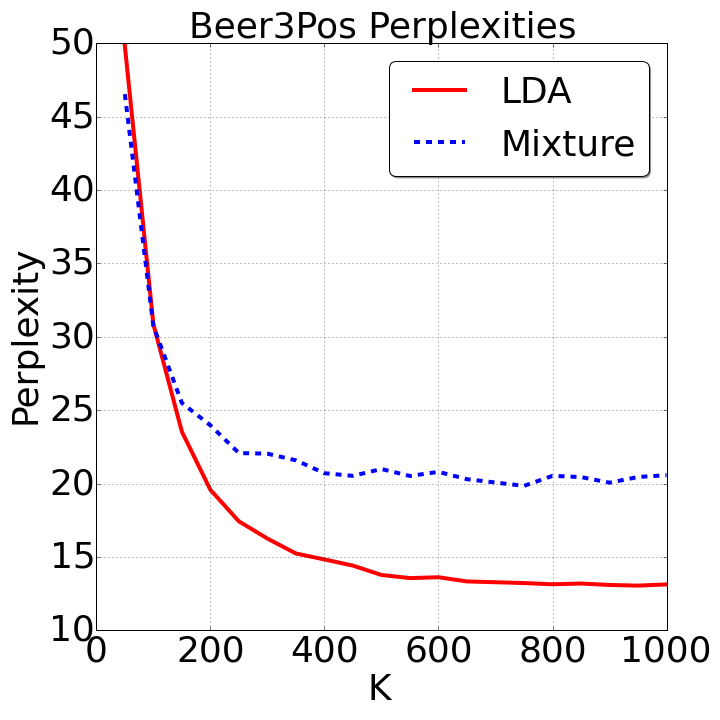
\includegraphics[width=0.5\linewidth]{07-lda/figures/perplexity.png}
\centering\caption{Results of model comparisons of LDA and multinomial mixture model on the beer3 positive ionization mode dataset. The lower perplexity values for $K>100$ demonstrates that LDA provides a better model fit on the held-out data when compared to the mixture model.\label{fig:m2lda-perplexity}}
\end{figure}

The perplexity results in Figure~\ref{fig:m2lda-perplexity} also suggest the appropriate value for K for the data to be in the range of 300 to 500 topics. These are the `elbow' point on the curve where increasing the number of topics does not result in any further decrease in perplexity. Following this, in Section~\ref{sub:lda-biological-findings}, we use $K=300$ for our detailed analysis on the biological significance of the results.

\subsection{Biological Findings\label{sub:lda-biological-findings}}

The MS2LDA workflow was independently applied to the four beer extracts. After pre-processing, we were left with around 1,000 MS peaks in both positive and negative ionization mode. Following the cross-validation experiments in Section~\ref{sub:lda-model-comparison}, 300 Mass2Motifs were extracted for each data file and checked for biochemical relevance. 30-40 Mass2Motifs in each of the positive ionization mode files were structurally annotated and diverse biochemically relevant substructures found included histidine, phenylalanine, adenine, hexose-units, and structural features such as water or carboxyl group loss.

The degree of Mass2Motifs (the number of spectra in which they occurred) varied from 1 to over 200 spectra, demonstrating the ability of MS2LDA to extract both generic and specific structural features. The number of Mass2Motifs within each spectrum also varied (around 600 spectra in each file consisted of one Mass2Motif, 300 of two, 50 of three, and 20 of four or more). Across the four files, an average of 70\% of spectra (Table~\ref{tab:ms2lda-coverage}) include at least one annotated Mass2Motif, demonstrating the power of MS2LDA for data reduction – i.e. annotating just 30-40 of the discovered Mass2Motifs provides biochemical insight into 70\% of the spectra. For comparison, we matched the spectra to the MassBank and NIST libraries (see Section S5.5) and obtained hits for only 25\% and 6\% of the MS2 spectra for NIST and MassBank, respectively, at a threshold of 90\% normalized scores. 

\begin{table}
\begin{centering}
\begin{tabular}{|c|c|c|c|}
\hline 
File & Total MS1 peaks & LInked to at least one structurally annotated M2M & \%\tabularnewline
\hline 
\hline 
Beer1Pos & 1282 & 951 & 74\tabularnewline
\hline 
Beer2Pos & 1567 & 1160 & 74\tabularnewline
\hline 
Beer3Pos & 1422 & 1055 & 74\tabularnewline
\hline 
Beer4Pos & 1363 & 930 & 68\tabularnewline
\hline 
\end{tabular}
\par\end{centering}
\caption{Mass2Motif coverage of MS1 peaks by percentage of MS1 peaks that can
be explained by at least one structurally annotated Mass2Motif for
the files acquired in positive ionization mode.\label{tab:ms2lda-coverage}}
\end{table}

\subsubsection{Automatic, Unsupervised, Chemical Substructure Discovery}

Mass2Motifs cover a diverse set of biochemical features, including amino acid related (i.e. histidine, leucine, tryptophan, and tyrosine), nucleotide related (i.e. adenine, cytosine, and xanthine), and other molecules such as cinnamic acid, ferulic acid, ribose and N-acetylputrescine. Mass2Motifs related to the same substructure or structural feature were consistently found across multiple beers (e.g. hexose-related Mass2Motifs were present in all positive ionization mode files with degrees from 58 to >100. Differences in degree and absence of some Mass2Motifs across the extracts show that MS2LDA also captures variability in metabolic composition of beer.

An example of ferulic acid (a compound present in cereals, an ingredient of beer) is given in Figure~\ref{fig:m2lda-ferulic-acid}. Three of the eleven spectra that include Mass2Motif 19 are shown. Conserved mass fragments are clearly visible across the three spectra with the most conserved highlighted in Figure ~\ref{fig:m2lda-ferulic-acid}D. Unlike existing software, e.g. MS2Analyzer \cite{ma2014ms2analyzer}, our method is unsupervised and has no need for prior knowledge about fragments of interest. It is of note that the neutral loss of the complete ferulic acid moiety was also included by MS2LDA, demonstrating that both fragments and losses can be present in a motif. It is able to extract a biochemically relevant pattern present in just 11 of the >1000 spectra, despite the fact that the individual spectra are quite different (see Section~\ref{sub:ms2lda-identification}).   

\begin{figure}[!htbp]
\centering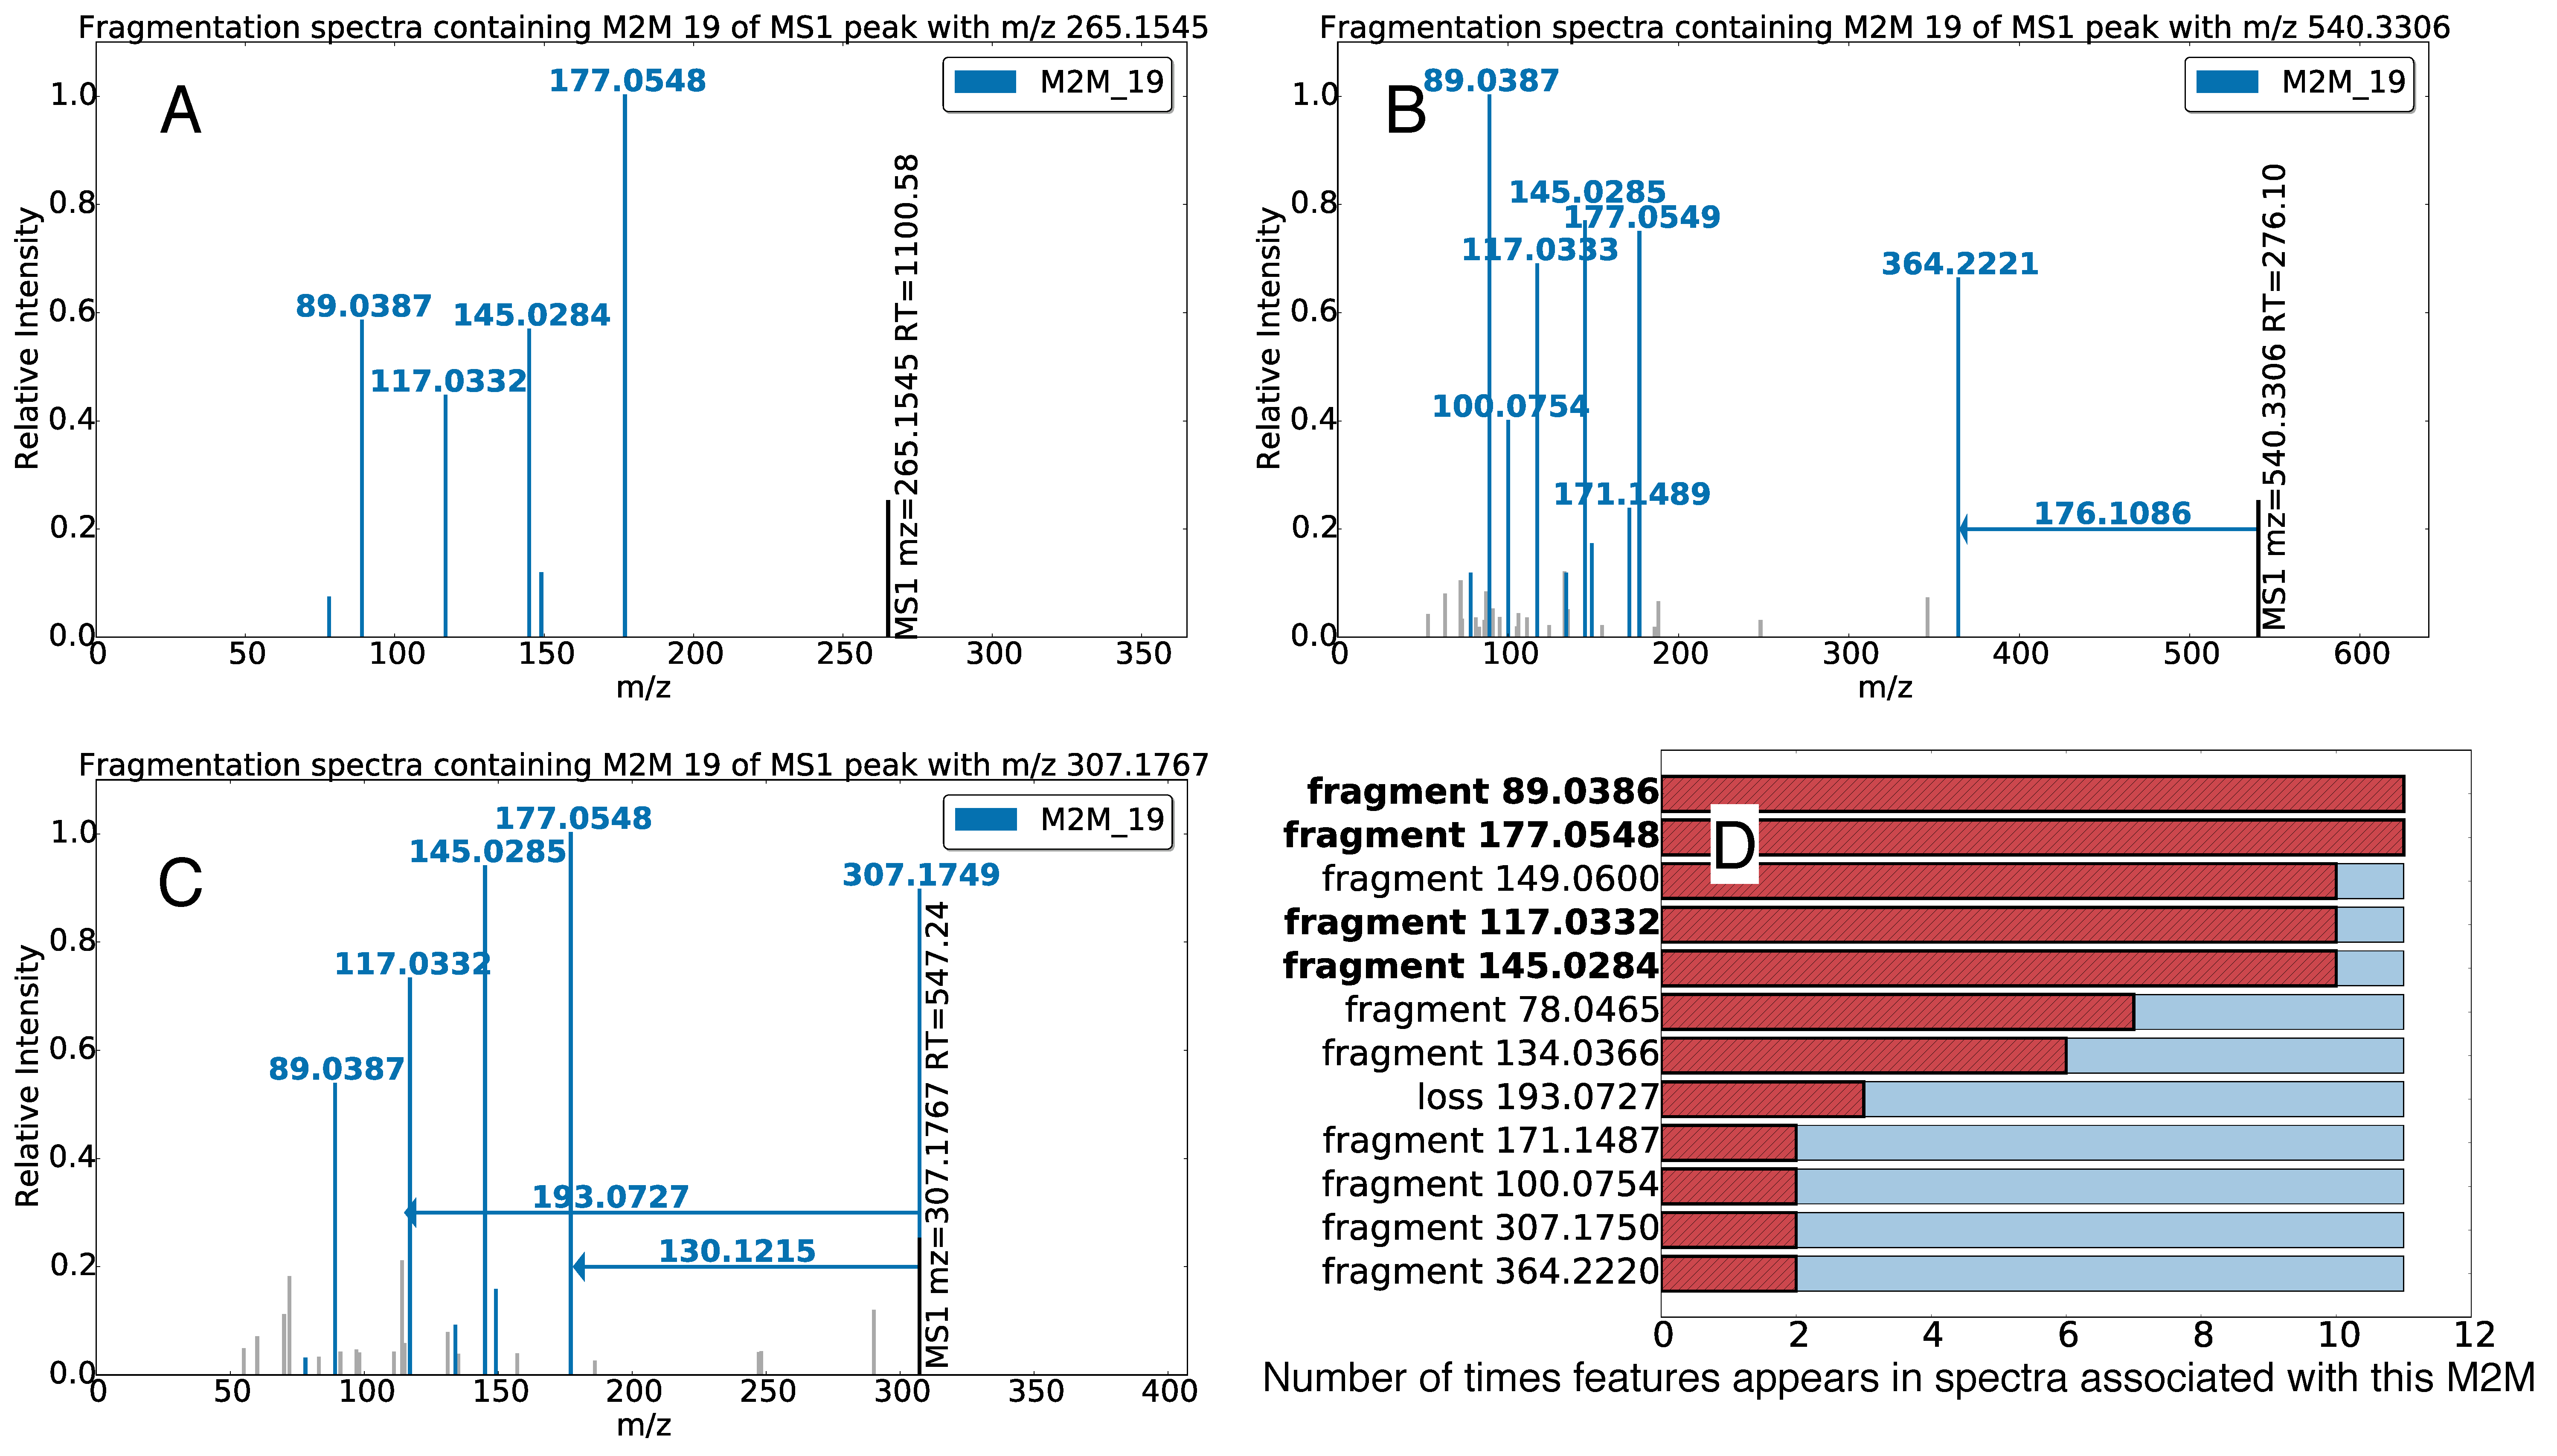
\includegraphics[width=1.0\linewidth]{07-lda/figures/ferulic_acid.pdf}
\centering\caption{Three spectra, from the beer3 positive ionization mode file, each of which includes Mass2Motif 19, annotated as the plant derived ferulic acid substructure. A-C highlight mass fragments and neutral losses (arrows originating at the precursor ions) included in Mass2Motif 19 (fragments not explained by Mass2Motif 19 are light grey). The histogram in D shows how common each fragment / loss is in the 11 instances of motif 19 found in the dataset. The abundant fragments with an m/z of 177.0545, 145.0284, 117.0332, and 89.0386 Da are most consistently present. It is of note that the neutral loss of 176.1086 and the protonated fragment of 177.0575 both relate to the complete ferulic acid substructure.\label{fig:m2lda-ferulic-acid}}
\end{figure}

\subsubsection{Structurally Annotated Mass2Motifs Validated in Authentic Standards}

Reference molecules present in the beer extracts can be identified based on chromatographic co-elution  and exact mass. As their identity is known, we can validate our structurally annotated Mass2Motifs. Of the 45 reference molecules we could identify, 38 included one or more annotated Mass2Motif, despite the fact that the original Mass2Motifs annotation was made independently of reference molecule characterization. 32 contained Mass2Motifs corresponding to known biochemical features.

Figure~\ref{fig:m2lda-standards} shows examples with fragmentation spectra colored by Mass2Motif. The spectra for phenylalanine (Figure~\ref{fig:m2lda-standards}A) and histidine (Figure~\ref{fig:m2lda-standards}B) share Mass2Motif 262, indicating the presence of a free (underivatized) carboxylic acid group. The loss of CHOOH (Mass2Motif 262) is in fact a common characteristic for many other underivatized amino acids and free organic acids and was associated with 10 of the 18 amino acids structures matched from the standards (the remaining 8 prefer alternative fragmentation routes – e.g. see the amine loss in tryptophan, Figure 3C). The other Mass2Motifs (115, 241) in Figures~\ref{fig:m2lda-standards}A and~\ref{fig:m2lda-standards}B are related to phenylalanine and histidine, respectively. Finally, Figure~\ref{fig:m2lda-standards}D is the MS2 spectrum of adenosine, which consists of an adenine molecule conjugated to a ribose sugar molecule. The two associated Mass2Motifs (156, 220) represent these two biochemically relevant structural features (i.e., adenine substructure and a loss corresponding to a ribose sugar).  

Spectra can include multiple Mass2Motifs. In each of Figures~\ref{fig:m2lda-standards}A to~\ref{fig:m2lda-standards}D, we observe two or more Mass2Motifs. We know of no other method that can do this without training spectra consisting of known structures, or a priori knowledge of interesting feature combinations. Multiple Mass2Motifs can also explain the same feature in one spectrum, i.e. the fragments 110.0717 (C5H8N3, [M+H]+)  and 120.0803 (C8H10N, [M+H]+) in Figures 3A and 3B are explained by Mass2Motifs 241 and 115 and also by the 46.0054 loss (CHOOH) of Mass2Motif 262. This demonstrates the manner in which MS2LDA decomposes molecules into their constituent building blocks, allowing for de novo metabolite annotation (see Section~\ref{sub:ms2lda-identification}). 

\begin{figure}[!htbp]
\centering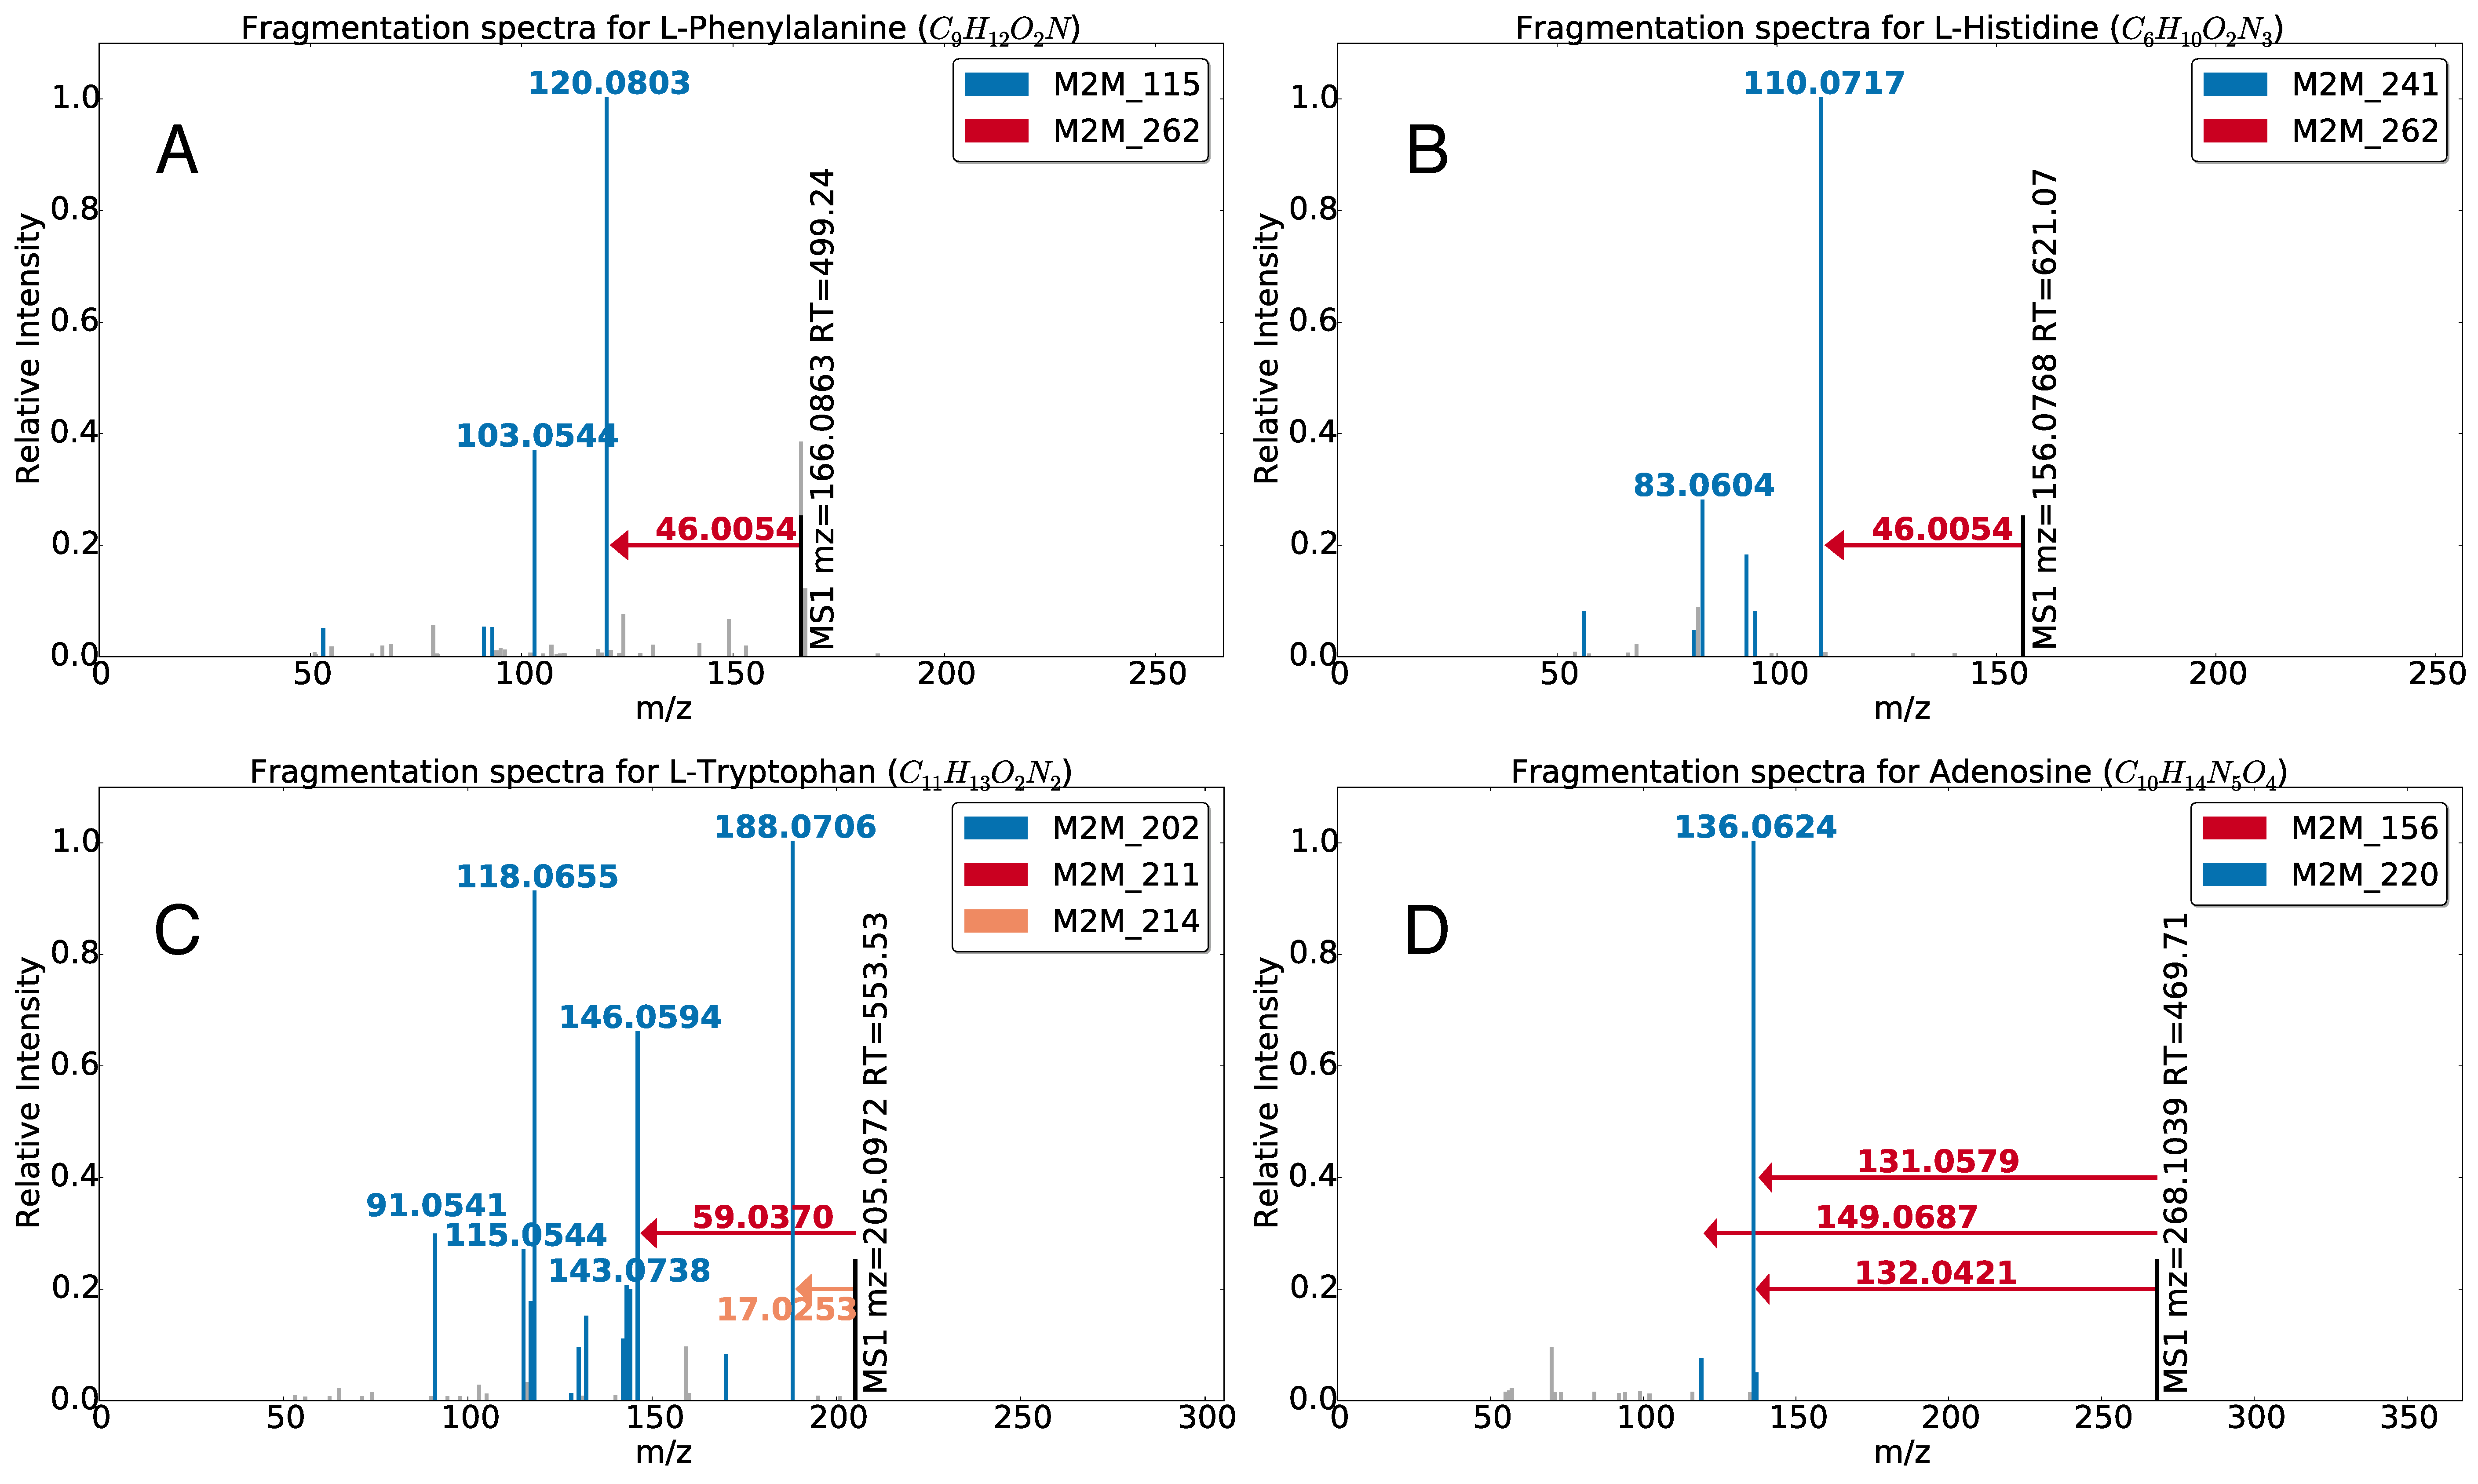
\includegraphics[width=1.0\linewidth]{07-lda/figures/standards.pdf}
\centering\caption{Mass2Motif spectra of identified metabolites A) L-histidine, B) L-phenylalanine, C) L-tryptophan, and D) adenosine. Characterized motifs (see Table~\ref{tab:ms2lda-standards}) are indicated by color.\label{fig:m2lda-standards}}
\end{figure}

% Preview source code for paragraph 1

\begin{table}
\begin{centering}
\begin{tabular}{| c | p{4cm} | c | p{4cm} | p{2.5cm} |}
\hline 
Mass2Motif & Annotation & Degree & Fragment or Loss Features & Elemental Formula\tabularnewline
\hline 
\hline 
115 & {[}phenylalanine-CHOOH{]}-based substructure.  & 28 & fragment\_120.0808, fragment\_103.0546, fragment\_91.0541 & C8H10N, C8H7, C7H7\tabularnewline
\hline 
156 & {[}ribose (pentose, C5-sugar)-H2O{]}-related loss.  & 22 & loss\_132.0421 & C5H8O4 \tabularnewline
\hline 
202 & {[}tryptophan-NH3{]}-related substructure.  & 15 & fragment\_118.0654, 
fragment\_117.0571, 
fragment\_91.0541, 
fragment\_130.0645,
fragment\_188.0706 & C8H8N, 
C8H7N, 
C7H7, 
C9H8N, C11H10NO2\tabularnewline
\hline 
211 & N-acetylputrescine substructure.  & 24 & loss\_59.0370, 
fragment\_114.0912, 
fragment\_72.0447, 
fragment\_60.0448 & C2H5NO, 
C6H12NO, C3H6NO, 
C2H6NO\tabularnewline
\hline 
214 & amine loss.  & 57 & loss\_17.0247  & NH3\tabularnewline
\hline 
220 & adenine substructure.  & 32 & fragment\_136.0629, 
fragment\_119.0351 & C5H6N5, 
C5H3N4\tabularnewline
\hline 
241 & histidine substructure.  & 21 & fragment\_110.0718, 
fragment\_156.0769, 
fragment\_93.0450, 
fragment\_95.0608 & C5H8N3, 
C6H10N3O2, 
C5H5N2, 
C5H7N2\tabularnewline
\hline 
262 & combined loss of H2O and CO \textendash{} indicative for free carboxylic
acid group (COOH).  & 90 & loss\_46.0053  & CH2O2 \tabularnewline
\hline 
\end{tabular}
\par\end{centering}
\caption{Annotations of the Mass2Motifs associated to the fragmentation spectra
of the standard peaks shown in Figure 3 of the paper. The degree of
a Mass2Motif indicates the number of MS2 fragmentation spectra in
the beer3 positive ionization mode data having fragment or loss features
that can be explained by the Mass2Motif (at the specified thresholding
level). \label{tab:ms2lda-standards}}
\end{table}

\subsubsection{Mass2Motifs Aid de-novo Metabolite Annotation\label{sub:ms2lda-identification}}

On average 70\% of the fragmented MS1 features are explained by at least one structurally annotated Mass2Motif (see Table~\ref{tab:ms2lda-coverage}) and can therefore be automatically classified. In a spectral matching comparison against the NIST MS/MS and MassBank databases on 7 of the metabolites annotated via the ferulic acid Mass2Motif, we found that only 1 returned a ferulic acid related hit, in spite of the clear presence of ferulic acid in all spectra (see e.g. Figure~\ref{fig:m2lda-ferulic-acid}). The Mass2Motif itself can be represented as a spectrum and be subjected to spectral matching, resulting in trans-ferulic acid as the best hit (hinting at the possibility of automatic Mass2Motif annotation). 

Spectra that are explained by the Mass2Motifs related to histidine, tyrosine, and tryptophan in Table~\ref{tab:ms2lda-standards} were also subjected to spectral matching. From 39 metabolites annotated by MS2LDA, 7 resulted in correct hits with another 8 producing structurally related hits. These results demonstrate the annotative power of MS2LDA, with which annotations can be made by matching only small portions of the spectra and therefore allowing annotation (classification) of molecules not present in databases. In summary, our method, adapted from text mining rather than developed explicitly for mass spectral data is able to annotate approximately three times as many metabolites as spectral matching. In addition, MS2LDA can annotate and group spectra based on neutral losses (e.g. the loss of CHOOH), which is not possible with spectral matching.

A key property of the LDA model for text is that a document can be described by one or more topics. Similarly in our MS2LDA workflow, a fragmentation spectrum can now be described by one or more Mass2Motifs. Figure~\ref{fig:m2lda-combined-m2m} demonstrates this with an example of a subset of the network produced by MS2LDAvis, consisting of molecules that include two Mass2Motifs (ferulic acid and ethylphenol). All but one molecule belongs to just one of the Mass2Motifs but one belongs to both (the fragments belonging to each Mass2Motif are clearly visible). The presence of both Mass2Motifs in this molecule allows us to putatively annotate it as feruloyltyramine (314.1386 m/z; [C18H20NO4]+) despite spectral matching producing no relevant hits. For comparison, the output of spectral clustering via Molecular Networking is shown on the right of Figure~\ref{fig:m2lda-combined-m2m}. This produces clusters interpretable as ferulic acid and ethylphenol related, but as each molecule belongs to one cluster, feruloyltyramine is assigned to the ethylphenol cluster and its relationship with ferulic acid is lost. 

%Allowing each spectra to include multiple Mass2Motifs thus gives far greater potential in making de novo structural annotations of molecules, rather than each parent ion having to be assigned to a single cluster alone. This is also shown in Figure S-14 where a matrix of cosine similarities of some parent ions drawn from the ferulic acid based cluster and the tyramine based cluster constructed through molecular networking is plotted. We see clear, distinct groupings of these spectra into two clusters based on the parent ions’ cosine similarities. Members of each cluster can therefore be explained by a single Mass2Motif (the ferulic acid cluster by M2M_19, and the tyramine cluster by M2M 58). However, one parent ion (the last row in Figure S-14) can also be explained by the two Mass2Motifs together. In cosine clustering, this parent ion would have to go into one cluster or the other based on its cosine similarity.

\begin{figure}[!htbp]
\centering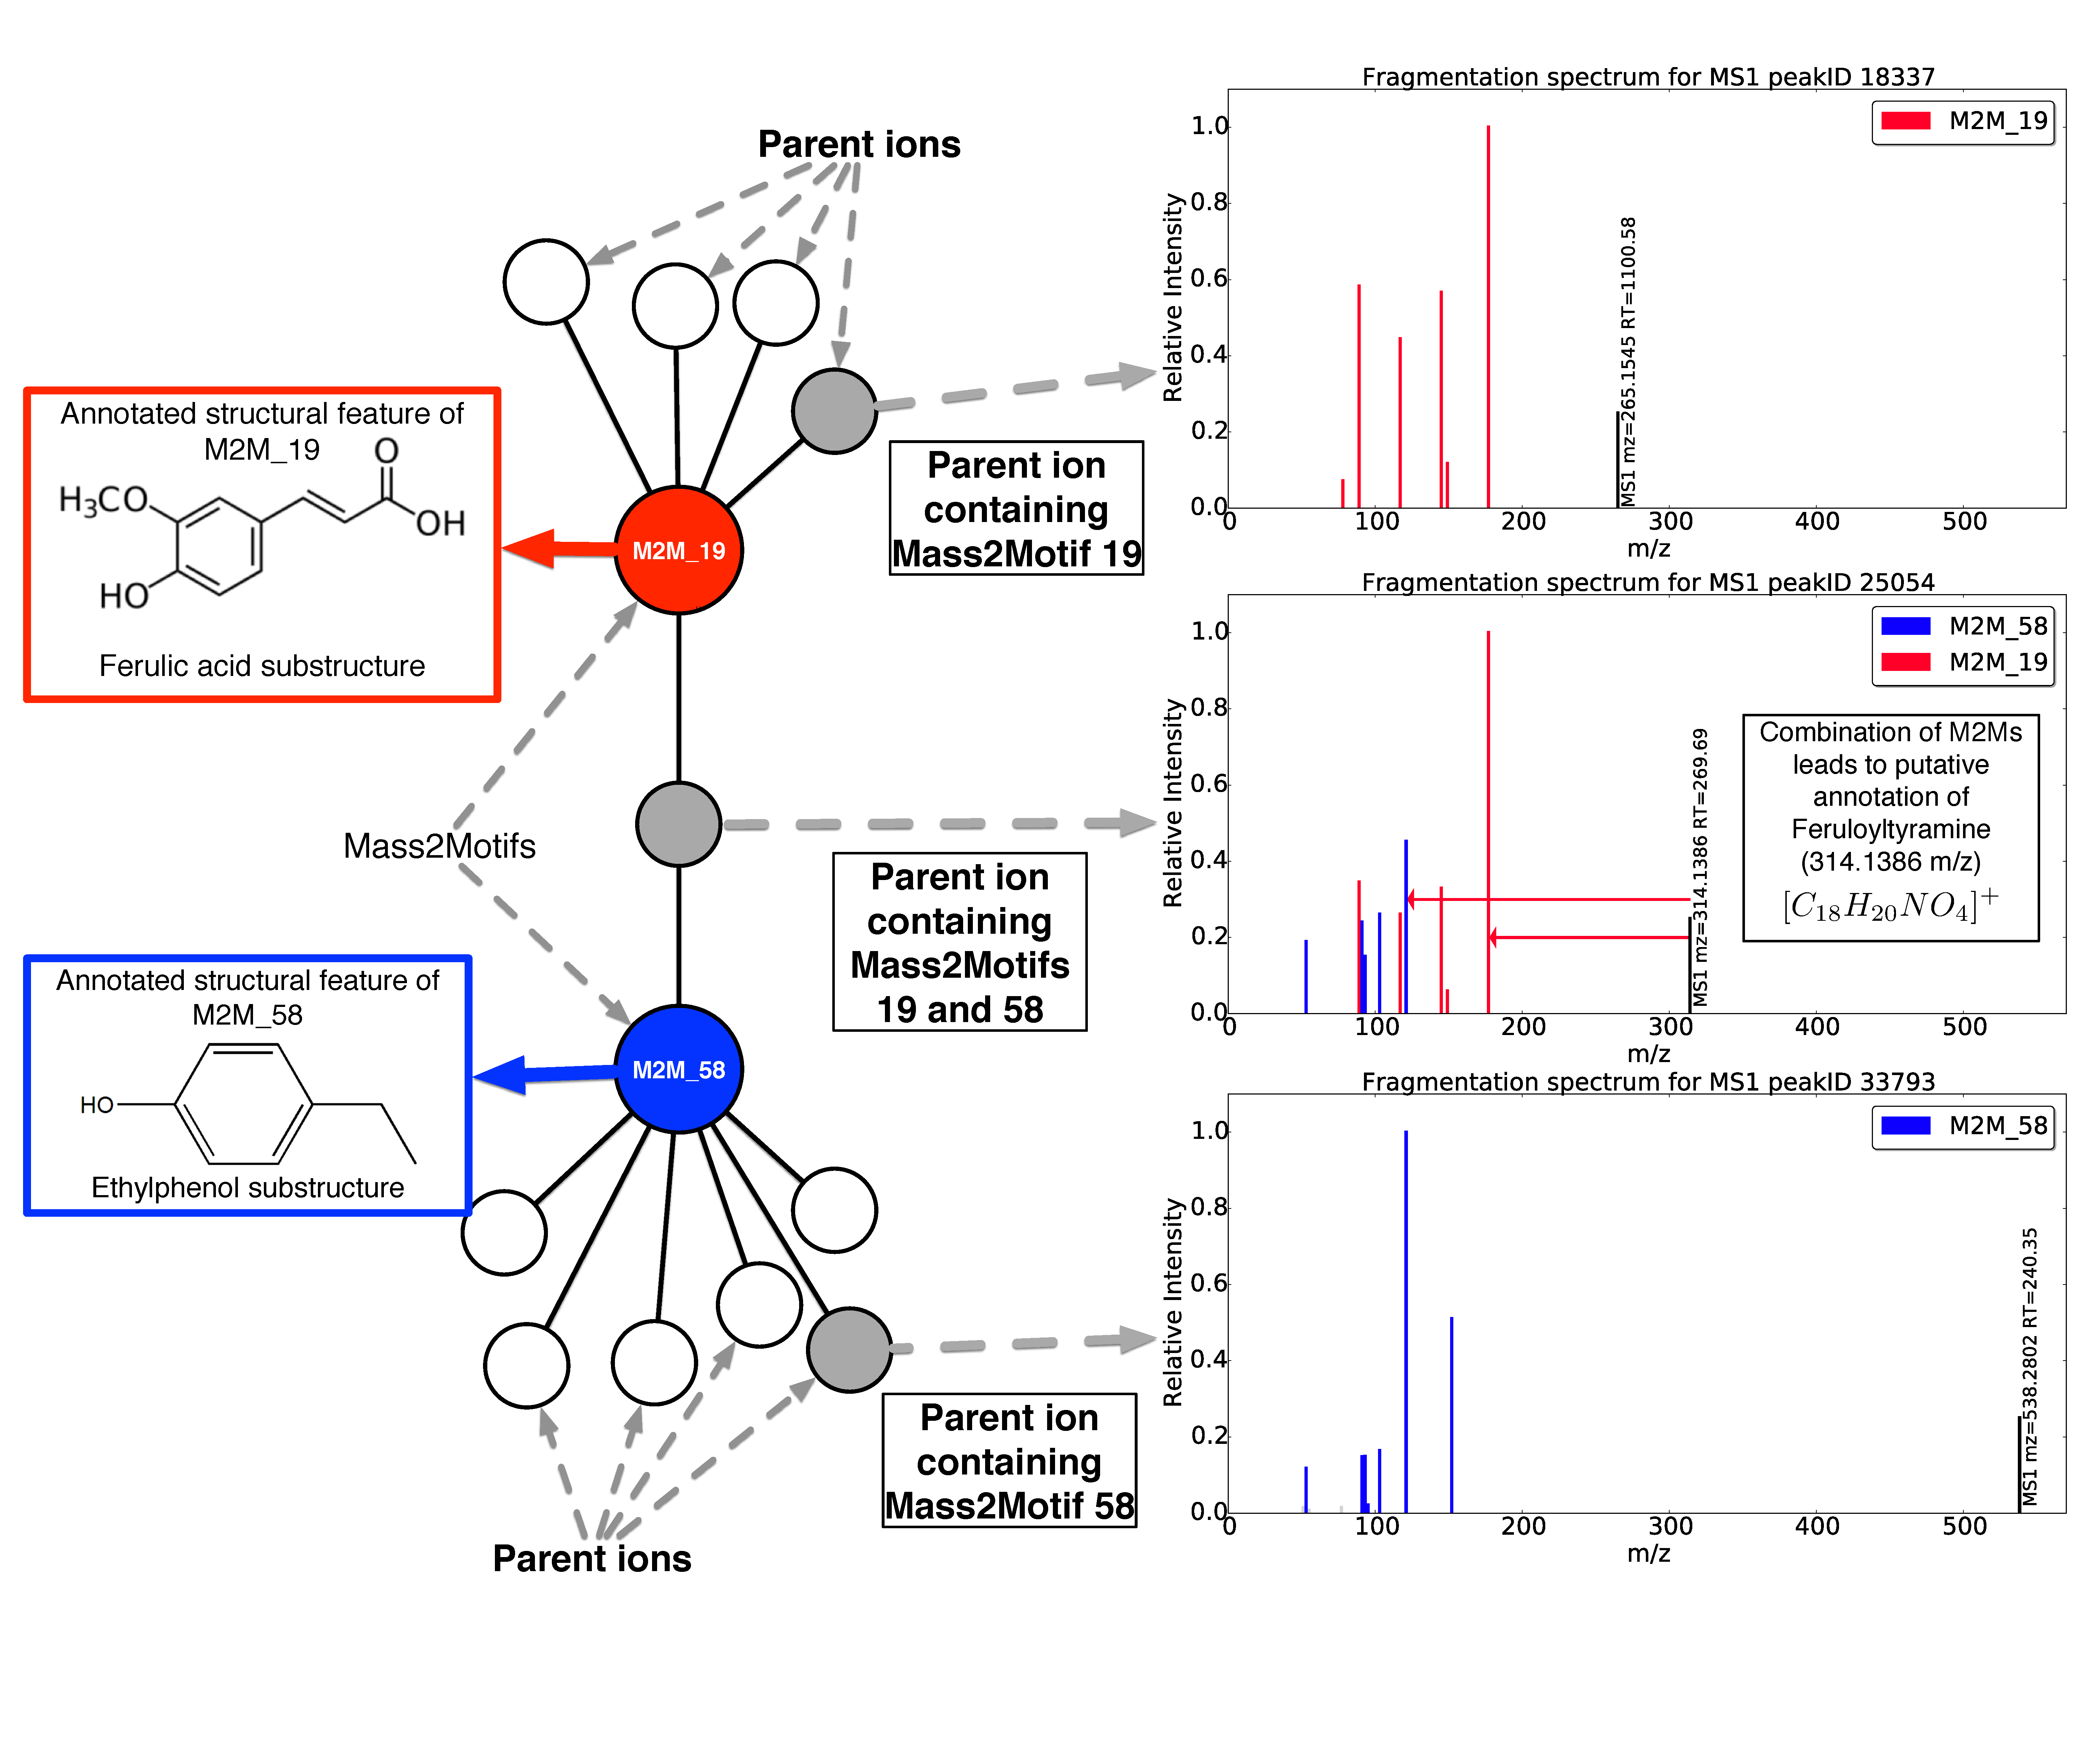
\includegraphics[width=1.0\linewidth]{07-lda/figures/combinedm2m.pdf}
\centering\caption{Mass2Motifs 19 and 58 were found to be representative of ferulic acid and ethylphenol, respectively. 11 and 42 MS1 features in the beer3 data set were explained by those two Mass2Motifs, respectively. Of those, one was explained by both Mass2Motifs, aiding in its annotation as feruloyltyramine (314.1386 m/z; [C18H20NO4]+). On the right of the plot, we show the clusters containing these three MS1 features created using the molecular networking tool (15) (top: ferulic acid, bottom: tyramine (ethylphenol)). The coloring of the nodes is dependent on their presence across the different beer extracts and the node size is proportional to the number of unique beer extracts the node fragmentation spectra are found in. The compound containing both Mass2Motifs is forced into the ethylphenol cluster, losing its relationship with ferulic acid.\label{fig:m2lda-combined-m2m}}
\end{figure}
 
\subsubsection{Differential Expression of Mass2Motifs Reveals Biochemical Changes Across Samples}

Being able to annotate more metabolites is beneficial when investigating the changes in metabolite intensity across multiple samples. As MS2LDA groups metabolites in a biochemically relevant manner, we can go a step further and consider the differential expression of Mass2Motifs in a manner similar to approaches taken in transcriptomics where it is common to consider the shared differential expression (DE) of a group of related transcripts as indicative of their contribution to a common aspect of cellular biology \cite{tarca2013comparison}. Using PLAGE \cite{tomfohr2005pathway}, we assessed the DE of each Mass2Motif based on the intensity changes of the relevant MS1 peaks between beers 2 and 3. Figure~\ref{fig:m2lda-heatmaps} shows MS1 intensities of metabolites including two Mass2Motifs with high PLAGE scores (note that for a high PLAGE score changes in expression do not need to be in the same direction). As an example of the kind of biochemical insight this provides, in Beer3, the free guanine (Figure~\ref{fig:m2lda-heatmaps}A) is more abundant whereas in Beer2, guanine-conjugates are more abundant. Similarly, the molecules associated to the pentose Mass2Motif (Figure~\ref{fig:m2lda-heatmaps}B) show DE between the extracts. It is the grouping performed by MS2LDA that exposes such insights from fragmentation data. We investigated whether or not similar outcomes can be achieved with with spectral similarity clustering. With this approach the 12 pentose-related metabolites were distributed across 10 clusters rather than appearing in a single grouping, hiding the potentially relevant correlated intensity change.

\begin{figure}[!htbp]
\centering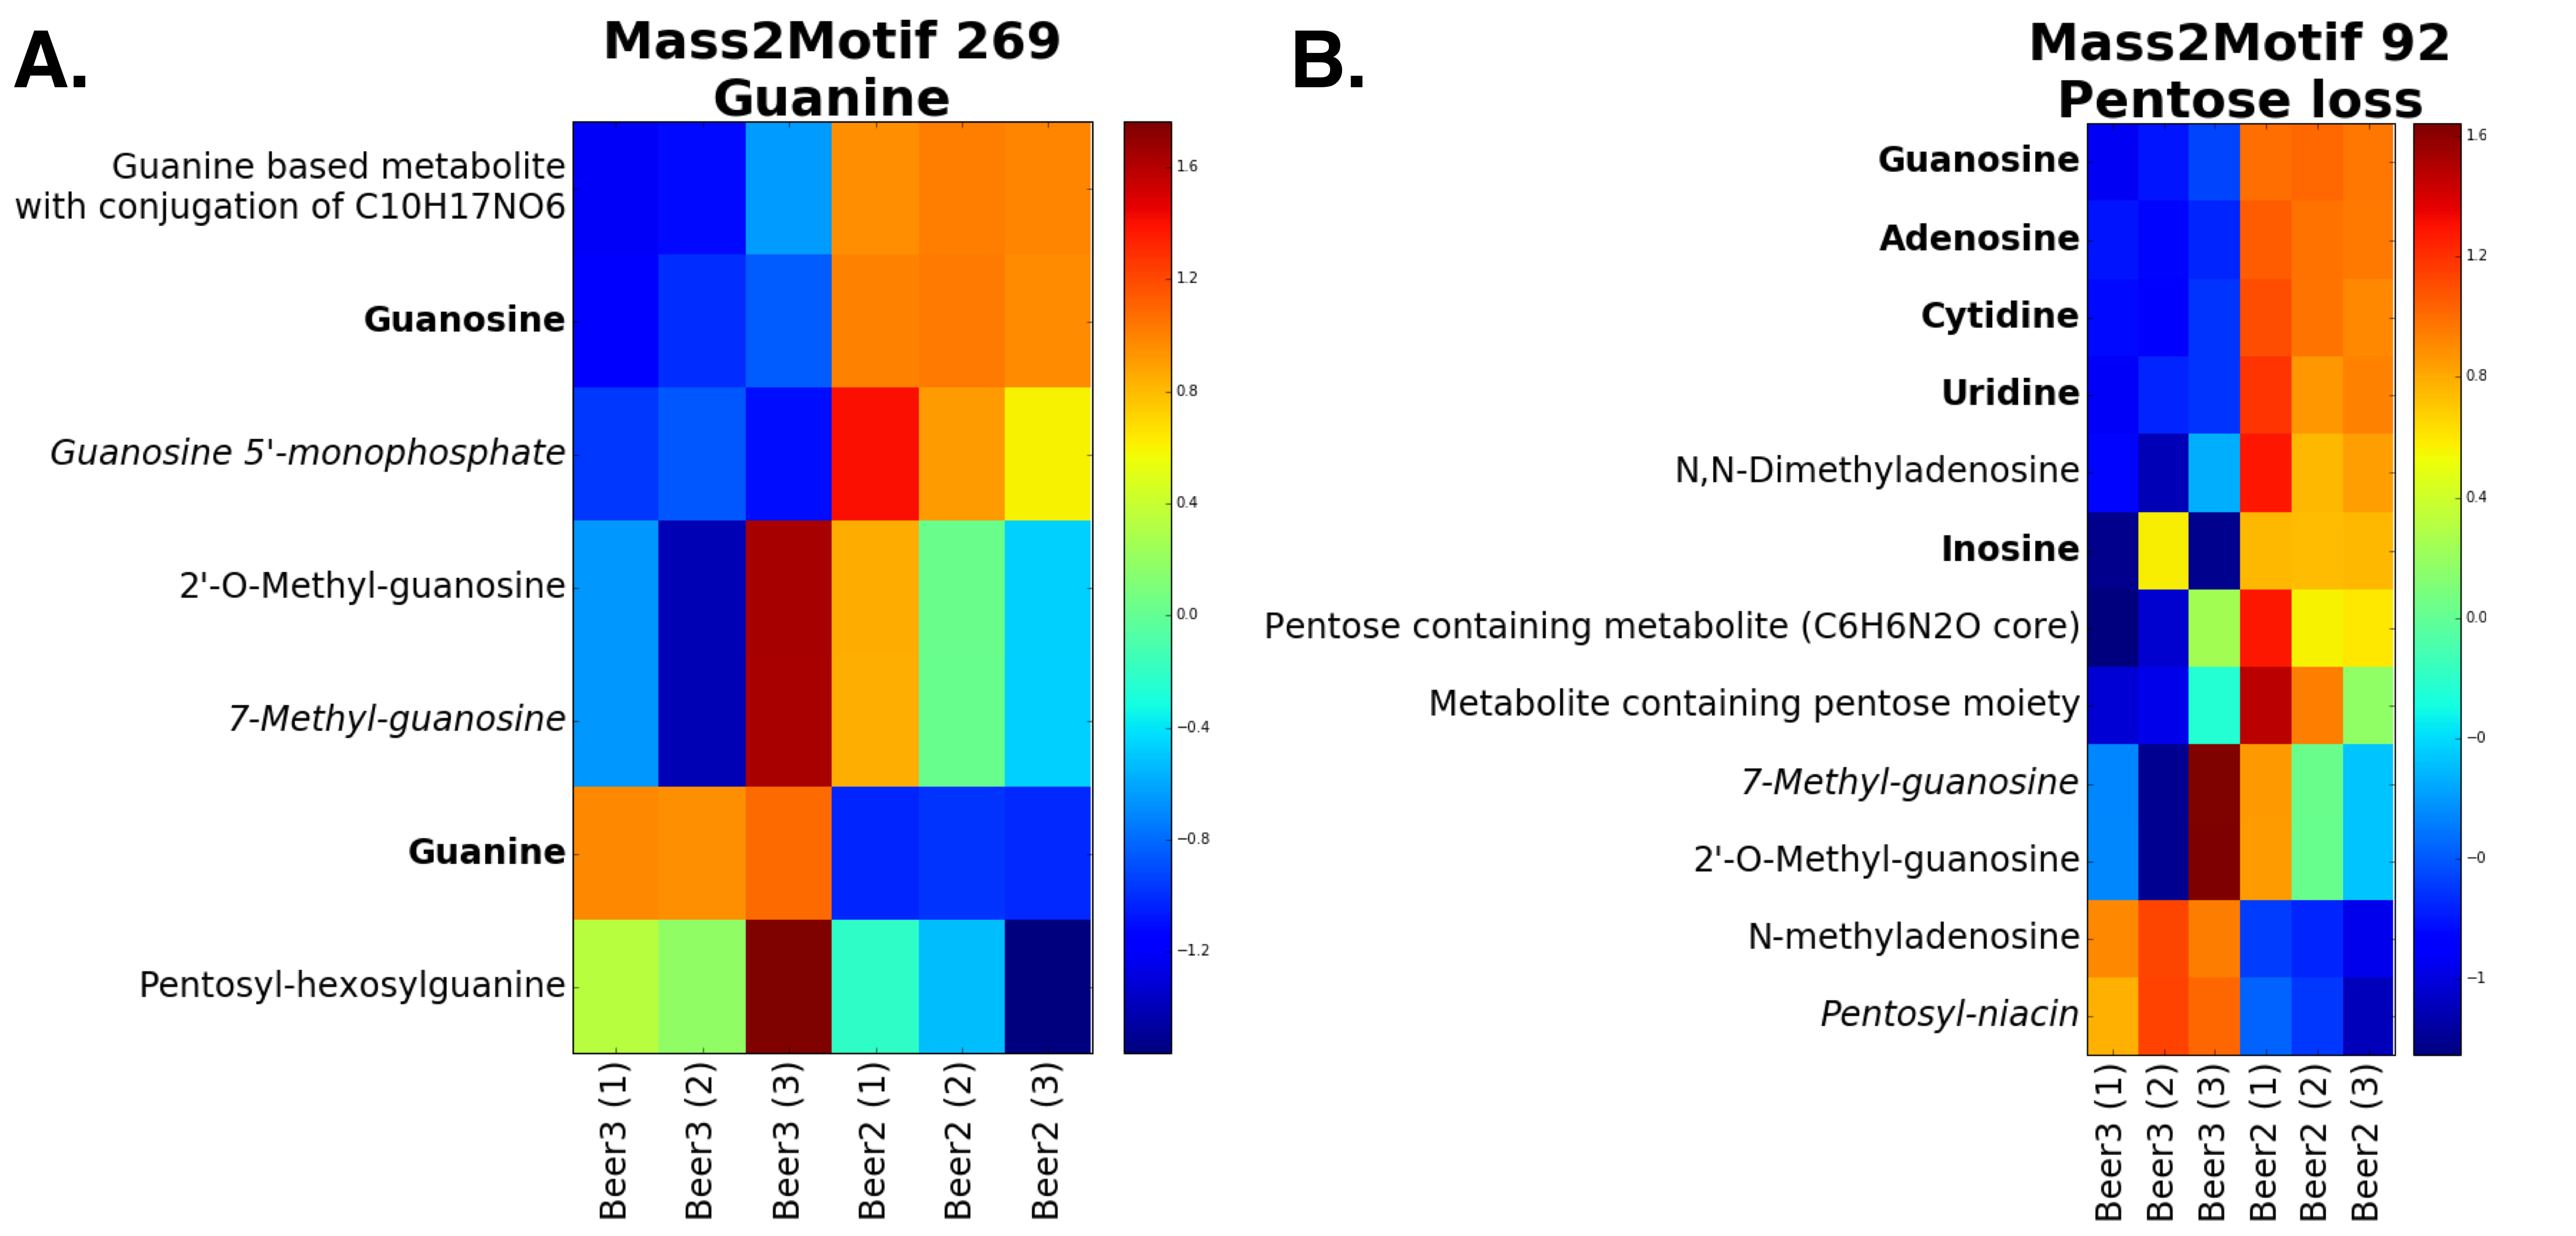
\includegraphics[width=1.0\linewidth]{07-lda/figures/heatmaps.png}
\centering\caption{Log fold change heat-maps for the A) guanine and B) pentose loss Mass2Motifs. Each row is an annotated MS1 peak and columns represent samples. Bold names could be matched to a reference compound.\label{fig:m2lda-heatmaps}}
\end{figure}

\section{Substructure Discoveries across Many Samples}

Manual inspection of the results revealed that many Mass2Motifs related to the same substructures were consistently present in two or more beers, despite each sample being processed independently. For example, the hexose-related Mass2Motifs were present in all positive ionization mode beer files with degrees from 58 to more than 100 in each beer. The results suggest that we can jointly model the presence or absence of Mass2Motifs across many samples at once.

\subsection{Extension to the LDA model}

\subsection{Results \& Discussion}

\section{Conclusion}